% Author: Jannes Bantje
% Modified: Lars Haalck lars.haalck@wwu.de
% please ask Lars Haalck first if you have any questions
%!TEX root = thesis.tex
% Author: Jannes Bantje
% Modified: Lars Haalck lars.haalck@wwu.de
% please ask Lars Haalck first if you have any questions

\documentclass[%
a4paper,
parskip=half,
index=totoc,
toc=listof,
fontsize = 10, %a5
%fontsize=11, %a4
headinclude,
twoside,
BCOR = 10mm, %a5
%BCOR=12mm, %a4
cleardoublepage=empty,
DIV=22, %a5
&DIV=13, %a4
numbers = noenddot,
%draft=false
final
]{scrreprt}


\usepackage[usenames,x11names]{xcolor}
\usepackage[final]{graphicx}
\usepackage{subcaption}
\usepackage[ngerman]{datetime}

% typographic settings, fonts, and math
\usepackage[utf8]{inputenc}
\usepackage[semibold]{libertine}
\usepackage[T1]{fontenc}
\usepackage{textcomp} % verhindert ein paar Fehler bei den Fonts
\usepackage[varl]{zi4}
\usepackage{mathtools,amssymb,amsthm} % Verbesserung von amsmath (die amsmath selbst lädt)
\usepackage[libertine,cmintegrals,bigdelims,varbb]{newtxmath}
\usepackage[ngerman]{babel}
\usepackage[babel=true, tracking=true,final]{microtype}

%eigene Packages hinzgefügt für Listings und Courier New als Schriftart für Variablen
\usepackage{courier}
\usepackage{listings}
\lstset{
        basicstyle=\ttfamily\normalsize,
        language = Python,
        breaklines = true,
        numbers=left,
        stepnumber=1,
        numbersep=10pt,
        frame = lines,
        %commentstyle = \color{white},
        %morecomment  = [l][\@gobble]{\#}, 
        %morecomment  = [is]{\"""}{\"""},
        breakatwhitespace = false,
}
\lstdefinestyle{intext}{
        basicstyle=\ttfamily\scriptsize,
        language = Python,
        breaklines = true,
        numbers=left,
        stepnumber=1,
        numbersep=10pt,
        frame = lines,
        %commentstyle = \color{white},
        morecomment  = [l][\@gobble]{\#}, 
        morecomment  = [is]{\"""}{\"""},
        breakatwhitespace = false,
}

%Package für Tabellen
\usepackage[normalem]{ulem}
\useunder{\uline}{\ul}{}
%weitere Abänderungen von mir für Verhinderung von Schusterjunge
\widowpenalty=10000
\clubpenalty=10000
\displaywidowpenalty = 10000

%Abänderungen Parametersatz
% \renewcommand{\topfraction}{0.9}
% \renewcommand{\bottomfraction}{0.8}

% \setcounter{topnumber}{2}
% \setcounter{bottomnumber}{2}
% \setcounter{totalnumber}{4}
% \setcounter{dbltopnumber}{2}
% \renewcommand{\dbltopfraction}{0.9}
% \renewcommand{\textfraction}{0.7}

% \renewcommand{\floatpagefraction}{0.7}
% \renewcommand{\dblfloatpagefraction}{0.7}

%Abänderung Lange/Kurze Version False = wenige Listings; True = alle Listings
\newif\ifimportant
\importanttrue



% set line spacing
\usepackage{setspace}
% for example 1.5 line spacing
\onehalfspacing

% literature settings
\usepackage[%
backend=biber,
sortlocale=auto,
natbib,
hyperref,
backref,
mincitenames=1,
maxcitenames=1,
style=ieee
]%
{biblatex}
\addbibresource{literature.bib} % sets literature file

% hyperref settings to make links clickable in PDF
\usepackage[%
hidelinks,
pdfpagelabels,
bookmarksopen=true,
bookmarksnumbered=true,
linkcolor=black,
urlcolor=SkyBlue2,
plainpages=false,
pagebackref,
citecolor=black,
hypertexnames=true,
pdfborderstyle={/S/U},
linkbordercolor=SkyBlue2,
colorlinks=false,
backref=false,
pdfencoding=auto,
psdextra
]{hyperref}
\hypersetup{final}

% enumeration settings
\usepackage[shortlabels]{enumitem}
\setlist[enumerate,description]{font=\sffamily\bfseries} % makes labels in enumeration bold
\usepackage[german=quotes]{csquotes}

\usepackage{ifdraft}
\setlength{\marginparwidth}{2.0cm}
\ifoptionfinal{}{
    % enable this line to better visualize overflows
    % \PassOptionsToPackage{showframe}{geometry}

    \paperwidth=\dimexpr \paperwidth + 3cm\relax
    \oddsidemargin=\dimexpr\oddsidemargin + 0cm\relax
    \evensidemargin=\dimexpr\evensidemargin + 3cm\relax
    \setlength{\marginparwidth}{2.5cm}
}

\usepackage[pass]{geometry}
% allows adding of todo notes at the side of the document
\usepackage[obeyFinal,textsize=small,textwidth=2.5cm]{todonotes}

% settings for the header and footer
\usepackage[headsepline=1pt]{scrlayer-scrpage}
\pagestyle{scrheadings}
\clearpairofpagestyles % clear defaults
\setkomafont{headsepline}{\color{gray}} % adds a gray line under the header
% set section title on the right, and chapter title on the left page in a double page
% document
\automark[section]{chapter}

\rohead{\rightmark} % section title on the right side
\lehead{\scshape\leftmark} % chapter title on the left side an in small caps
\ofoot[\pagemark]{\pagemark} % page marks always on the outer site of the page

\setcounter{secnumdepth}{4}
\setcounter{tocdepth}{4}


% sets page marks and footer and header texts to sans-serif in gray
\renewcommand*{\pnumfont}{\sffamily}
\renewcommand*{\footfont}{\sffamily\color{gray}}
\renewcommand*{\headfont}{\sffamily\color{gray}}

% change the chapter, section and subsection font sizes and spacings a bit for a5 format
% \setlength{\footskip}{1.75\baselineskip} % change the spacing a bit for a5 format
% \RedeclareSectionCommand[%
% afterskip=1\baselineskip,%
% beforeskip=-1\baselineskip]{chapter}

\setkomafont{chapter}{\LARGE}
\setkomafont{section}{\Large}
\setkomafont{subsection}{\large}

% adds a thick gray line after the chapter number
\renewcommand*{\chapterformat}{%
    \thechapter\enskip
    \textcolor{gray!50}{\rule[-\dp\strutbox]{1.5pt}{\baselineskip}}\enskip
}

% math environments
\usepackage{amsthm}
\usepackage{thmtools}
\usepackage{mdframed}
\usepackage{blindtext}
\renewcommand{\listtheoremname}{Übersicht aller Aussagen}

% -- Theoreme als PDF-Lesezeichen
\usepackage{bookmark}
\bookmarksetup{open,numbered}
\makeatletter
\newcommand*{\theorembookmark}{%
   \bookmark[
     dest=\@currentHref,
     rellevel=1,
     keeplevel,
   ]{%
     \thmt@thmname\space\csname the\thmt@envname\endcsname
     \ifx\thmt@shortoptarg\@empty
     \else
       \space(\thmt@shortoptarg)%
     \fi
   }%
}
\makeatother

% -- Definition der einzelnen Umgebungen
\declaretheoremstyle[%
     headfont=\sffamily\bfseries,
     notefont=\normalfont\sffamily,
     bodyfont=\normalfont,
     headformat=\NAME\ \NUMBER\NOTE,
     headpunct=,
     postheadspace=\newline,
     spaceabove=\parsep,spacebelow=\parsep,
     %shaded={bgcolor=gray!20},
     postheadhook=\theorembookmark,
     mdframed={
         backgroundcolor=gray!20,
             linecolor=gray!20,
             innertopmargin=6pt,
             roundcorner=5pt,
             innerbottommargin=6pt,
             skipbelow=\parsep,
             skipbelow=\parsep }
     ]%
{mainstyle}

\declaretheoremstyle[%
     headfont=\sffamily\bfseries,
     notefont=\normalfont\sffamily,
     bodyfont=\normalfont,
     headformat=\NAME\ \NUMBER\NOTE,
     headpunct=,
     postheadspace=\newline,
     spaceabove=15pt,spacebelow=10pt,
     postheadhook=\theorembookmark]%
{mainstyle_unshaded}

\declaretheoremstyle[%
     headfont=\sffamily\bfseries,
     notefont=\normalfont\sffamily,
     bodyfont=\normalfont,
     headformat=\NUMBER\NAME\NOTE,
     headpunct=,
     postheadspace=\newline,
     spaceabove=15pt,spacebelow=10pt,
     % shaded={bgcolor=gray!20},
     postheadhook=\theorembookmark]%
{mainstyle_unnumbered}

\declaretheorem[name=Definition,parent=section,style=mainstyle]{definition}
\declaretheorem[name=Definition,numbered=no,style=mainstyle]{definition*}
\declaretheorem[name=Definition,sharenumber=definition,style=mainstyle_unshaded]{definitionUnshaded}

\declaretheorem[name=Theorem,sharenumber=definition,style=mainstyle]{theorem}
\declaretheorem[name=Theorem,numbered=no,style=mainstyle_unnumbered]{theorem*}

\declaretheorem[name=Proposition,sharenumber=definition,style=mainstyle]{proposition}
\declaretheorem[name=Lemma,sharenumber=definition,style=mainstyle]{lemma}

\declaretheorem[name=Satz,sharenumber=definition,style=mainstyle]{satz}
\declaretheorem[name=Satz,sharenumber=definition,style=mainstyle_unshaded]{satzUnshaded}
\declaretheorem[name=Satz,numbered=no,style=mainstyle_unnumbered]{satz*}

\declaretheorem[name=Korollar,sharenumber=definition,style=mainstyle]{korollar}

\declaretheorem[name=Notation,numbered=no,style=mainstyle_unnumbered]{notation}
\declaretheorem[name=Bemerkung,numbered=no,style=mainstyle_unnumbered]{bemerkung}
\declaretheorem[name=Beispiel,numbered=no,style=mainstyle_unnumbered]{beispiel}
\declaretheorem[name=Beispiele,numbered=no,style=mainstyle_unnumbered]{beispiele} 


%Informationen zur Arbeit
\newcommand{\printname}{Timo Lietmeyer}
\newcommand{\printnumber}{459 169}

\newcommand{\printtitle}{Formbasiertes Objekttracking \\ mit der Discrete Curve Evolution}
\newcommand{\printalttitle}{Shape-based object tracking \\ with the Discrete Curve Evolution}
\newcommand{\printcity}{Münster}
\newcommand{\printtype}{Bachelorarbeit}
\newcommand{\printdegree}{Bachelor of Science}
\newcommand{\printsupervisor}{Dr. Christian Knoth}
\newcommand{\printfirstassessor}{Prof. Dr. Reinhard Moratz}
\newcommand{\printsecondassessor}{Dr. Christian Knoth}
\newcommand{\printinstitute}{Fachbereich Geowissenschaften \\
    Institut für Geoinformatik}

% !!!only for pseudo text, can be deleted!!!
\usepackage{blindtext}

\hypersetup{pdfinfo = {
	Title={Formbasiertes Objekttracking mit der Discrete Curve Evolution},
	Author=\printname,
	Keywords = {Discrete Curve Evolution, DCE, YOLO, Bachelorarbeit, Thesis, \printdegree, Formbasiertes Objekttracking mit der Discrete Curve Evolution, Formbasiertes Objekttracking}}}

\begin{document}
% set the pager numbering to big roman numbers for firt few pages
\pagenumbering{Roman}
\listoftodos


% titlepage does not need cleardoubleoddemptypage
\begin{titlepage}
	%!TEX root = ../thesis.tex
\thispagestyle{empty}

\begin{center}
    
\includegraphics[height=1.7cm]{logos/wwu.pdf}
    \hfill
    \raisebox{-1.5ex}{
\includegraphics[height=1.7cm]{logos/ifgi_logo.png}}
    \par
    \vspace*{8ex}
    {
        \linespread{0.9}
        \LARGE
        \printtitle
        \par
    }
    \normalsize
    \vspace*{8ex}
    \large
    \textsc{\printtype}\\
    \normalsize
    zur Erlangung des akademischen Grades\\
    \large
    \textsc{\printdegree}
    \par
    \normalsize
    \vspace*{6ex}
    Westfälische Wilhelms-Universität Münster\\
    \printinstitute
\end{center}

\par
\vspace*{6ex}
Erstgutachter:\\
\large
\textit{\printfirstassessor}

\par
\normalsize
\vspace*{2ex}
Zweitgutachter:\\
\large
\textit{\printsecondassessor}

\par
\normalsize
\vspace*{2ex}
Eingereicht von: \\ %\hspace{4cm} Matrikelnummer: \\
\large
\textit{\printname} \\ %\hspace{4cm} \textit{459 169}\\

% \par
% \normalsize
% \vspace*{6ex}
% Matrikelnummer:\\
% \large
% \textit{459 169}




\par
\normalsize
\vspace*{4ex}
\printcity, \today %\makeatletter
% \monthname
% \makeatother~\the\year

\end{titlepage}

\begin{titlepage}
	%!TEX root = ../thesis.tex
\thispagestyle{empty}
\LARGE
% \vspace*{\fill}
\vspace*{2em}
\begin{center}
    \printtitle
    \par
    \par\noindent\rule{0.8\textwidth}{0.4pt}
    \par
    \printalttitle
\end{center}
% \vspace*{\fill}

\end{titlepage}

%!TEX root = ../thesis.tex
\begin{abstract}
\section*{Abstract}
\todo{muss noch ein bisschen weiter ausgebaut werden}
In dieser Arbeit wird ein Ansatz zu formbasiertem Objekttracking mit der Discrete Curve Evolution (DCE) vorgestellt. Zu Detektion der Objekte wird maschinelles Lernen in Form von YOLO verwendet. Das Objekttracking kann mit einem Formähnlichkeitsmaß für jedes Polygon bewertet werden. Es wird eine prototypische Implementierung beschrieben, die auf der Programmiersprache Python basiert. Die Evaluation des Ansatzes erfolgt an mehreren Testvideos mit verschiedenen YOLO-Modellen. Im Rahmen dieser Arbeit zeigt sich, dass das Formähnlichkeitsmaß eine geringe Abweichung von ca. 5 Grad pro Winkel aufweist, was ein Objekttracking ermöglicht. Damit kann die DCE zu einem Objekttracking beitragen.

\end{abstract}

\cleardoubleoddemptypage

\tableofcontents
\cleardoubleoddemptypage

% set the page numbering back to arabic
\pagenumbering{arabic}
\setcounter{page}{1}
%!TEX root = ../thesis.tex
\chapter{Einleitung}
\label{ch:intro}

 \todo{siehe und s. immer gleich benutzen (entweder ausschreiben oder nur s.)}
\section{Motivation}{ 
	
Durch die Verfügbarkeit von Open-Source Software, die neuronale Lernverfahren verwendet und eine sehr schnelle Objekterkennung auf Videoströmen anbietet, lassen sich viele relevante Anwendungen in der Geoinformatik realisieren, beispielsweise im Bereich der Verkehrsüberwachung. \\
In der Arbeitsgruppe \glqq Theoretische und kognitive Grundlagen der Geoinformatik \grqq{} am Institut für Geoinformatik der Universität Münster ist es geplant mit einem hybriden Ansatz Anwendungsmöglichkeiten solcher Systeme zu verbessern. Dabei soll eine geometrische Analyse Ergebnisse der neuronalen Erkennung verifizieren, um das Risiko von Fehldetektionen zu minimieren. Unsere Hypothese vermutet, dass der Ansatz der Discrete Curve Evolution (DCE) von \citet{Latecki1999a}  eine wichtige Stufe sein kann. Diese Vermutung basiert auf Vorarbeiten von \citet*{Dorr2015} an der Universität Maine.
}



\section{Zielsetzung und Forschungskontext}
{%Forschungskontext Reintext
Der Forschungskontext besteht als Basis aus dem Paper von \citeauthor*{Dorr2015}. Bei \citeauthor*{Barkowsky2000} wird die DCE zur Vereinfachung von geometrischen Strukturen auf Karten verwendet \citep{Barkowsky2000}. \\
Weitere Anwendungsfälle sind die Vereinfachung von Skeletten \citep{Latecki2007}, die automatische Kartierung von Entwässerungsnetzen anhand der Geländetopografie mit der Unterstützung der DCE zur Erkennung relevanter Punkte \citep{ZHENG201517} oder auch der medizinische Bereich. Im letzteren kann die DCE bei der Analyse von MRI (Magnetic Resonance Images) helfen \citep{Supot2007}. Des Weiteren kann die DCE bei Gesten- und Handdetektion mit einem Kinect Sensor eingesetzt werden \citep{Lai2016}. Ein ähnlicher Anwendungsfall zu dieser Arbeit, der sich damit beschäftigt nur die relevante Frames aus einem Video zu extrahieren, um die Frames per Second (\glqq Bilder pro Sekunde\grqq{}, FPS) zu minimieren, wurde von \citeauthor*{Latecki2000a} bereits erprobt \citep{Latecki2000a}. \\


Ziel dieser Arbeit ist es ein prototypisches System zu entwickeln, welches Objekte in Videomaterial detektiert und deren Umrisse vereinfacht. Diese Objektumrisse können dann in ihrer Ähnlichkeit verglichen werden, um einzuschätzen, ob die Objekte trackbar sind. Der Ablauf des Programmes ist folgendermaßen geplant. \\ 
Zur Evaluation wird Videomaterial von Autobahnen aufgenommen, welches im Rahmen der Bachelorarbeit analysiert wird. Ein beispielhafter Verlauf anhand eines einzelnen Bildes ist in Abb. \ref{Bsp_Dorr} zu sehen. \\
Die folgenden Schritte werden für jeden Frame im Video ausgeführt. 
Als ersten Schritt müssen die zu erkennenden Objekte detektiert werden. Dies kann mit der Schwellwertsegmentierung nach Otsu erfolgen, da die Objekte eindeutig zu erkennen sind \citep{Otsu1979}. Außerdem ist die Schwellwertsegmentierung sehr ressourcenschonend, da kein maschinelles Lernverfahren verwendet wird. Eine andere Methode mit einem maschinellen Lernverfahren wäre die Benutzung von YOLO zur Segmentierung. Beide Verfahren beinhalten das Umwandeln in eine Binärmaske als zweiten Schritt. Diese Binärmaske wird im dritten Schritt in ein Polygon umgewandelt, welches mit der DCE vereinfacht wird. Dem Maschinellen Lernverfahren YOLO wird gegenüber der Schwellwertsegmentierung den Vorzug gegeben, da die ersten beiden Schritte Detektierung und das Erzeugen der Binärmaske, bzw. des Umrisses der Objekte, bereits in YOLO integriert sind.\\
Die DCE berechnet anhand eines Grenzwertes, welche Punkte für die Darstellung einer Form irrelevant sind, sodass diese ohne größeren Informationsverlust entfernt werden können \citep{Barkowsky2000}. Dadurch wird eine bedarfsbezogene Vereinfachung, anhand eines festen Grenzwertes, des Polygons ermöglicht. 
Weiterhin kann die Vereinfachung die mit dem DCE Algorithmus erreicht wird, eine Überprüfung der Ergebnisse vereinfachen. Hierfür bietet sich Verwendung eines Formähnlichkeitsmaßes für Polygone an. \\
Die Ergebnisevaluation ist durch eine Auswertung des Formähnlichkeitsmaßes möglich. Wenn dieses Maß den entsprechenden Wert hat, kann beurteilt werden, ob Objekttracking mit der DCE möglich ist. Außerdem ist eine visuelle Beurteilung des Videos, welches als Endprodukt entsteht, möglich.\\}
\begin{figure}[ht]
	\vspace{-0.5cm}
	   \centering
	   \includegraphics*[scale = 0.5, keepaspectratio, trim=2 2 2 2 ]{images/Example_bird.png}
	   \caption[Beispielablauf der Segmentierung und DCE]{Beispielablauf einer Vereinfachung mit der DCE \citep{Dorr2017}.}
	   \label{Bsp_Dorr}
\end{figure}


% \todo{mussn noch ausformuliert werden}
% Forschungskontext:
% \begin{itemize}
% 	\item Vereinfachung von Karten (Geometrische Strukturen) \citep{Barkowsky2000}
% 	\item Skeletvereinfachungsmethode \citep{Latecki2007}
% 	\item Kombinierung DCE und Skeleton Construction Technik \citep{ZHENG201517}
% 	\item Medizinischer Kontext MRI \citep{Supot2007}
% 	\item DCE auf digitale Bilder (Videos ) \citep{Latecki2000}
% 	\item Gesten (Fingertips) und Handdetection basierend auf DCE mit Kinect Sensor \citep{Lai2016}
% 	\item DCE Grundlagen \citep{Latecki1998}
% \end{itemize}
\section{Aufbau der Arbeit} \todo{muss überarbeitet werden (Begründung für weitere TR hier ein?)}
{Diese Bachelorarbeit ist in 6 Kapitel aufgeteilt. \\ 
Der Theoretische Hintergrund wird zuerst beschrieben. Dieser enthält eine Einführung in den YOLO-Algorithmus mit einer kurzen Erläuterung der Grundlagen im Maschinellen Lernen, sowie eine Erklärung der Theorie hinter der Discrete Curve Evolution. Außerdem wird die genutzte Programmiersprache definiert und die externen Bibliotheken beschrieben. Des Weiteren werden weitere vom Programm genutzte Algorithmen erklärt und ein kurzer Meta-Ablauf des Programmes skizziert. \\
Die Implementierung bildet mit der Evaluation den Hauptteil der Arbeit. Ersteres beschreibt den Programmablauf an ausgewählten Codebeispielen und zeigt Änderungen im Rahmen der Implementierung zum Theoretischen Hintergrund auf. Die Evaluation ordnet die Ergebnisse verschiedener Testdurchläufe ein. Die Diskussion benennt Gründe für die gewonnenen Ergebnisse der Evaluation. \\
Nach diesem Abschnitt wird ein Fazit gezogen. Der Ausblick in dem Weiterentwicklungen zum Thema dieser Arbeit erläutert werden, schließt diese Arbeit ab. }





\cleardoubleoddemptypage

%!TEX root = ../thesis.tex
\chapter{Objekterkennung mit neuronalen Netzen}
\label{ch:Theoretischer Hintergrund}
% {Die Einführung in den theoretischen Hintergrund dieser Arbeit umfasst die Erläuterung der Aufbereitung der Daten mit einem Maschinellem Lernverfahren, namens YOLO, und eine Einführung in die \glqq Discrete Curve Evolution\grqq{}. Beide Verfahren werden im Rahmen dieser Arbeit miteinander kombiniert.
% }



%\section{\glqq You Only Look Once\grqq{}(YOLO)}
{
	
	\section{Der YOLO Algorithmus \label{subsec:YOLO_Alg}} 
	{Da der Blick des Menschen Objekterkennung, -einordnung und -wirkung intuitiv ermöglicht, ist es unserem Gehirn im Zusammenspiel mit unseren Augen möglich, schnell und genau zu sehen. Durch diese Fähigkeiten können wir mit nur wenig bewussten Gedanken komplexe Aufgaben, wie Fahrradfahren bewältigen, bei denen gleichzeitig mehrere Sinne beansprucht werden. \citep{Redmon2016}. \\
	Dem Computer kann dies mit schnellen und genauen Algorithmen zur Objekterkennung beigebracht werden. Aktuelle Systeme nutzen Klassifikatoren zur Objekterkennung. Dieser wird an verschiedenen Stellen in variablen Skalierungen im Testbild angewendet, um eine Klassifizierung eines Objektes zu ermöglichen \citep{Redmon2016}. \\ 
	
	\begin{figure}[ht]
		\centering
		\includegraphics*[scale = 1, keepaspectratio, trim=2 2 2 2 ]{images/YOLO/YOLO_detection_system.png}
		\caption[Das YOLO Objekterkennungsystem]{Das YOLO Objekterkennungsystem \citep{Redmon2016}}
		\label{YOLO_Objectdetection}
 	\end{figure}\glqq You Only Look Once\grqq{} (YOLO) betrachtet Objekterkennung als einzelnes Regressionsproblem, indem direkt von Bildpixel zu Boundingbox Koordinaten und Klassenwahrscheinlichkeiten berechnet wird. Dieser Algorithmus analysiert nur einmal ein Bild und sagt direkt vorher, welche Objekte wo vorhanden sind. Dadurch ist die Komplexität des  Aufbaus von YOLO sehr gering, wie in Abb. \ref{YOLO_Objectdetection} zu sehen \citep{Redmon2016}. \\
	Die Performance zur Objekterkennung wird durch das Training von YOLO mit vollständigen Bildern gesteigert. Durch dieses vereinheitlichte Modell entstehen mehrere Vorteile gegenüber den traditionellen Objekterkennungssystemen \citep{Redmon2016}. \\
	Der erste Vorteil von YOLO ist die gesteigerte Performance. Dies wird dadurch ermöglicht, dass Objekterkennung auf Bildern als Regressionproblem betrachtet wird und deshalb keine komplexe Pipeline die Verarbeitung eines Bildes verlangsamt.  \citep{Redmon2016}. 
	Zweitens analysiert YOLO ein Bild global mit Vorhersagen zur Objekterkennung. Dadurch kann YOLO beim Verwechseln von Hintergrund und Objekten im Vordergrund um die Hälfte im Vergleich zu Fast R-CNN verringern. Dies geschieht vor allem durch den größeren Kontext, den YOLO durch die Gesamtbildanalyse gewinnt \citep{Redmon2016}. \\
	Der dritte Vorteil ist das YOLO mit generalisierten Repräsentationen von Objekten trainiert wurde um die Fehlertoleranz bei der Anwendung auf neue Bereiche und unerwartete Eingaben zu vergrößern, aufgrund der Möglichkeit der hohen Verallgemeinerung \citep{Redmon2016}. \\
	Ein Nachteil von YOLO liegt in der Genauigkeit. Der Algorithmus hat Schwierigkeiten einige, insbesondere kleine, Objekte genau zu lokalisieren \citep{Redmon2016}. \\
	Da der Quellcode, mehrere vortrainierte Modelle und die Trainingsdaten von YOLO Open Source sind und zum Download bereitstehen, ist dieser Algorithmus für den Rahmen dieser Arbeit leicht zugänglich und anwendbar \citep{Redmon2016}. \\

	YOLO unterteilt in Bild in $S \times S $ Rasterzellen. Wenn der Mittelpunkt eines Objektes in eine Rasterzelle fällt, ist diese für die Erkennung des Objektes zuständig. Boundingboxen und ihre jeweiligen Confidence Scores werden für jede Rasterzelle vorhergesagt \citep{Redmon2016}.
	Der Confidence Score beschreibt, wie sicher sich das Modell ist, dass die Boundingbox ein Objekt dieser Klasse enthält und für wie genau das Modell diese Vorhersage hält. \\
	Dieser hier berechnete Wert enthält nicht nur die Wahrscheinlichkeit, dass diese Klasse in der Bounding Box vorkommt, sondern auch wie gut die vorhergesagte Box mit dem detektierten Objekt überein stimmt. Ein Beispielablauf ist in Abb. \ref{YOLO_Model} zu sehen.
	\begin{figure}[ht]
		\centering
		\includegraphics*[scale = 2, keepaspectratio, trim=2 2 2 2 ]{images/YOLO/YOLO_model.png}
		\caption[Das YOLO Modell]{Das YOLO Modell\citep{Redmon2016}}
		\label{YOLO_Model}
 	\end{figure}

	


	Da jede Rasterzelle nur 2 Bounding Boxen vorhersagen und eine Klasse haben kann, unterliegt YOLO einer räumlichen Einschränkung. Dies begrenzt die Anzahl der benachbarten Objekte, die das Modell vorhersagen kann. Außerdem ist es für das Modell schwierig, kleine Objekte, die in Gruppen auftreten zu detektieren \citep{Redmon2016}. \\
	Eine weitere Herausforderung ist, dass Objekte mit neuen oder ungewöhnlichen Formen auftreten können und dadurch die Vorhersage erschwert wird. Da die Netzwerkarchitektur aus mehreren 'Downsampling' Schichten besteht, benutzt das Modell relativ grobe Features zur Vorhersage der Bounding Boxen \citep{Redmon2016}. \\
	Außerdem sorgt das Training mit einer Verlustfunktion (für eine Erklärung s.  Formel \ref{YOLO_Loss_function}, S. \pageref{YOLO_Loss_function} und Abb.  \ref{YOLO_loss_function_detail}, S. \pageref{YOLO_loss_function_detail}), die die Erkennungsleistung annähert, dafür dass Fehler bei kleinen Bounding Boxen genauso wie bei großen Bounding Boxen behandelt werden. Dies ist ein Nachteil, weil ein kleiner Fehler in einer großen Box meistens wenig Auswirkungen hat, aber ein kleiner Fehler in einer kleinen Box eine sehr viel größer Auswirkung auf die IOU hat. Falsche Lokalisierungen sind eine weitere Hauptfehlerquelle \citep{Redmon2016}. \\
	YOLO ist für den Anwendungszweck dieser Arbeit geeignet, weil der Algorithmus die entsprechende Performance und einfache Verfügbarkeit von trainierten Modellen bietet. Außerdem existieren mehrere weitere Versionen (s. Abb. \ref{YOLO_timeline_vers}, S. \pageref{YOLO_timeline_vers}) von YOLO, die Vorteile in einzelnen Aspekten bieten \citep{Terven2023}. Zuvor war angedacht eine Schwellwertsegmentierung \citep{Otsu1979}, bspw. nach \citeauthor{Otsu1979}, zur Objektdetektion zu verwenden, da diese Methode ressourcenschonender ist. Dieser Ansatz wurde jedoch verworfen, weil die Implementierung den Rahmen dieser Arbeit übersteigen würde.\\

	Y
	Im Rahmen dieser Arbeit wird YOLOv8 von Ultralytics verwendet. Diese bietet Vorteile in der Performance und Genauigkeit der Objektdetektierung. 
	} 

	\section{YOLOv8 von Ultralytics}{ \label{subsec:YOLOv8_theoretic}
	
	Im Januar 2023 wurde von der Firma Ultralytics YOLOv8 veröffentlicht, welches auf YOLOv5 basiert. Diese Version beinhaltet 5 verschiedene Modelle (YOLOv8n (nano), YOLOv8s (small), YOLOv8m (medium), YOLOv8l (large), YOLOv8x (extra large)), die mit unterschiedlich großen Datensätzen trainiert wurden  \citep{Terven2023}. \\	
	Ein Vorteil dieser YOLO Implementierung ist, dass verschiedene Varianten für Objektdetektion, -segmentierung und -verfolgung, sowie -klassifizierung existieren. In dieser Arbeit wird hauptsächlich die \grqq -seg\glqq{}-Variante verwendet, welches bereits eine Segmentierung der Umrisse der detektierten Objekte integriert hat.
	\begin{figure}[h]
		\centering
		\includegraphics*[scale = 0.20, keepaspectratio]{images/YOLO/YOLOv8_object_detector_general.png}
		\caption[Architektur modernen Objektdetektoren]{Architektur modernen Objektdetektoren \citep{Terven2023}}
		\label{YOLO_obj_det_gen}
	\end{figure}
	Die Architektur dieser Algorithmen kann man in 3 Teile aufteilen (s. Abb. \ref{YOLO_obj_det_gen}). Dies sind der Backbone, der Neck und der Head \citep{Terven2023}. \\
	Das Detektieren nützlicher Features vom Eingabebild geschieht im Backbone, welcher meist als CNN implementiert ist \citep{Terven2023}. \\
	Zwischen Backbone und Head wird der Neck eingesetzt, um die Features, die der Backbone ausgibt, zu aggregieren und zu verfeinern. Der Fokus liegt auf der Verbesserung der räumlichen und semantischen Informationen über die unterschiedlichen Skalierungen hinweg \citep{Terven2023}. \\
	Die letzte Komponente ist der Head, welcher die Vorhersagen, aufgrund der von dem Backbone und Neck gelieferten Features, trifft. Hier werden meistens aufgabenspezifische Teilnetze eingesetzt, um Klassifizierung, Lokalisierung und auch sofortige Segmentierung durchzuführen. Aus den Features, die der Neck liefert, erstellt der Head Vorhersagen für jeden Objektkandidaten. Ein Post-Procressing Schritt, wie die Non-Maximum-Supression (NMS), filtert überlappende Vorhersagen heraus, sodass nur die sichersten Detektionen genutzt werden \citep{Terven2023}.\\
	Da YOLOv8 auf YOLOv5 basiert, wird in diesem ein ähnlicher Backbone genutzt. Für die Architektur von YOLOv8 s. Abb. \ref{YOLOv8_Arch} (S. \pageref{YOLOv8_Arch}). 

	Um die Performance insbesondere bei der Objekterkennung von kleineren Objekten zu verbessern, nutzt YOLOv8 CloU \citep{Zheng2020} und DFL \citep{Li2020} Verlustfunktionen für Boundingboxloss und binäre Kreuzentropie für Klassifizierungsloss \citep{Terven2023}. \\

	Mit dem YOLOv8-Seg Modell wird auch eine Variante angeboten, die semantische Segmentierung ermöglicht. Dieses Modell wird in dieser Arbeit genutzt, da es den Anforderungen entspricht.
	}
}

\cleardoubleoddemptypage

%!TEX root = ../thesis.tex
\chapter{Formverarbeitung}

\section{Discrete Curve Evolution (DCE)}
\label{sec:Discrete Curve Evolution}
{Die \glqq Discrete Curve Evolution\grqq{} (DCE, \cite{Latecki1999a,Latecki1999c}) ist eine Methode zur Polygonvereinfachung, die die Formähnlichkeit des Polygons beibehält und 1999 von Longin Latecki und Rolf Lakämper vorgestellt wurde (\citep{Barkowsky2000,Latecki1999a,Latecki1999c}). Im Folgenden wird diese Methode genauer erläutert. 
\\
Die Vereinfachung von Polygonen, während die Form der Polygone erkennbar bleibt und kleinere Knicke verschwinden, ist die wichtigste Eigenschaft der DCE. Dies basiert auf der schrittweisen Entfernung von Punkten, die den geringsten Beitrag zur Form des Polygons leisten. Dieser Beitrag des einzelnen Punktes zur Form des Polygons kann in einem Relevanzmaß gemessen werden \citep{Barkowsky2000}. 
\\
\begin{figure}[ht]
	   \centering
	   \includegraphics*[scale = 0.8, keepaspectratio, trim=2 2 2 2 ]{images/DCE/schem_maps_paper_kinks.png}
	   \caption[Beispielpolygone für die Erläuterung der Relevanz des Knicks]{Beispielpolygone für die Erläuterung der Relevanz des Knicks. Die fettgedruckten Knicke stellen die betrachteten Liniensegmente dar \citep{Barkowsky2000}.} 
	   \label{Bsp_Rev_Measur_K}
\end{figure} In Abbildung \ref{Bsp_Rev_Measur_K} ist ein Beispiel zu sehen. Bei diesen Formen sind die Knicke durch den Fettdruck zu erkennen. Der Knick in (a) kann als irrelevante Formänderung interpretiert werden, während die Knicke in (b) und (c) deutlich stärker zu erkennen sind. Diese beiden Knicke leisten einen relevanten Beitrag zur Form des Polygons. Der Knick in (d) hat jedoch den größten Anteil an der Form des Beispielobjektes \citep{Barkowsky2000}. 
\\
Diese Unterschiede zum Beitrag eines einzelnen Punktes zur Form eines Polygons lässt sich durch existierende geometrische Konzepte erklären. Wenn man den Knick in Abbildung \ref{Bsp_Rev_Measur_K} (a) mit (b) vergleicht, ist zu erkennen, dass (b) den gleichen Winkel hat wie (a). Der Unterschied ist jedoch, dass die Strecken bei (b) länger sind. Dies erhöht den Beitrag des Punktes in (b) zur Form des Polygons im Vergleich zu dem Punkt in (a).
Der Knick in (c) hat einen größeren Winkel im Vergleich zu (a). Die Länge der Strecken ist jedoch gleich. Bei dem Knick in (d) ist deutlich zu erkennen, dass dieser den signifikantesten Anteil zur Form des Polygons leistet. Dies ist durch den größten Winkel in Verbindung mit den längsten Strecken zwischen Punkten gegeben \citep{Barkowsky2000}.
\\
Dieses Beispiel zeigt, dass die Relevanz jedes Knicks für ein Polygon durch den Winkel und die Länge der an den Punkt anschließenden Liniensegmente definiert werden kann. Je größer der Winkel und die Länge der Liniensegmente sind, desto wichtiger ist der Beitrag des Knicks zur Form der Kurve. Aus diesen Beobachtungen kann eine Funktion K gebildet werden, die den Beitrag eines Knicks zur Form des Polygons misst. Diese sollte monoton steigend sein, wenn die Länge der benachbarten Liniensegmente wächst und der Winkel größer wird \citep{Barkowsky2000}.
\\
Eine formale Definition dieser Funktion kann folgendermaßen erfolgen. Zwei konsekutive Liniensegmente werden als $S_1, S_2$ definiert. Das Maß für die Relevanz des Knicks K, welches aus $S_1 \cup S_2$, dem Winkel  $\beta(S_1, S_2)$ am Scheitelpunkt von $S_1,  S_2$ und den Längen von $S_1, S_2$ besteht, kann nach folgender Formel berechnet werden (nach \citet{Latecki1999a}):
\\
\begin{equation}
	K(S_1,S_2) = \frac{\beta(S_1,S_2)l(S_1)l(S_2)}{l(S_1) + l(S_2)} 
	\label{Equ_K_Bark} 
\end{equation}
 Hier ist $l$ als Funktion definiert, welche die Länge des Segments berechnet. \\
 Der Vorteil dieser Formel ist, dass je höher der Wert von $K(S_1, S_2)$ ist, desto größer ist der Beitrag des Knicks von $S_1 \cup S_2$ zur Form des Polygons \citep{Barkowsky2000}.
 \\
 Nun wird der Prozess der \glqq Discrete Curve Evolution\grqq{} beschrieben.\\ Das Minimum der Kostenfunktion \ref{Equ_K_Bark} ergibt ein Tupel von Liniensegmenten, welches durch eine einzelne Linie ersetzt wird, indem ihre Endpunkte verbunden werden. Dies beschreibt eine Iteration der DCE. Dies wird für jede sich daraus neu ergebene Form wiederholt, indem $K$ für jeden Punkt immer neu berechnet wird \citep{Barkowsky2000}.
 \\ 
 Letztendlich ist die DCE folgendermaßen aufgebaut. Der kleinste Wert von $K(S_1,S_2)$ definiert in jedem Iterationsschritt das Paar von konsekutiven Liniensegmenten $S_1, S_2$, welches durch ein einzelnes Liniensegment von den Endpunkten $S_1 \cup S_2$ ersetzt wird. Das Relevanzmaß $K$ wird lokal für jeden Iterationsschritt der DCE neu berechnet und ist deshalb eine lokale Eigenschaft der Form des ursprünglichen Polygons. \\ Die DCE ermöglicht, wie in den Abbildungen \ref{Bsp_DCE_Bark_Paper} (S. \pageref{Bsp_DCE_Bark_Paper}) und \ref{Scr:DCE_test_run_nrw} (S. \pageref{Scr:DCE_test_run_nrw}) zu erkennen, die Substitution kleinerer Knicke ohne den Gesamteindruck der Form des Polygons nachhaltig zu verändern \citep{Barkowsky2000}.
 \\
 Ein weiterer Vorteil dieses Algorithmus ist, dass er immer terminiert, da in jedem Iterationsschritt die Zahl der Punkte um eins reduziert wird. Die DCE konvergiert für geschlossene Polygone gegen einen Zustand, wo nur noch drei Liniensegmente im Polygon vorhanden sind. Durch einen Abbruch des Prozesses ist es jedoch möglich, ein Polygon auf eine bestimmte vorgegebenen Punktanzahl zu reduzieren.\citep{Barkowsky2000}. \\ 
 Für die Anwendung in dieser Arbeit ist die DCE wegen ihrer geringen Komplexität sehr gut geeignet.
}

\section{Formähnlichkeitsmaß (NICHT FERTIG)}{ \label{theo:SSM}
	\todo{Klare Benennung Formähnlichkeitsmaß oder Formähnlichkeitsmesswert}
	Zur Evaluation des Objekttrackings wird ein Formähnlichkeitsmaß (\glqq Shape Similarity Measure\grqq{}, SSM) genutzt, welches die Winkel der Polygone vergleicht. \\
	Da ein von DCE vereinfachtes Polygon sich von Frame zu Frame nicht ändert, kann die Winkeldifferenz der Polygone voneinander subtrahiert werden. Diese Subtraktion muss als Absolutbetrag erfolgen, um bei der folgenden Aufsummierung aller Winkeldifferenzen eines Polygons im Vergleich zum nächsten, einen Wert zu erhalten, welcher gegen 0 geht. Um die Möglichkeit zu finden, wo beide Polygone die höchste Formähnlichkeit haben, muss ein Polygon rotiert werden. Ohne die Verwendung des Absolutbetrages würde bei einer Rotation stets das gleiche Ergebnis als Winkeldifferenzgesamtssumme berechnet werden, weil bei der Addition der einzelnen Winkeldifferenzen zur Gesamtwinkeldifferenzsumme das Kommutativgesetz gilt. Die höchste Formähnlichkeit wird durch die geringste Winkeldifferenzgesamtssumme beim Vergleich der Polygone repräsentiert.\\
	In der Formel \ref{equ:SSM} ist dies dargestellt. Das Summenzeichen selbst steht für die Winkeldifferenzgesamtssumme,$n$ für die Anzahl der Punkte im Polygon, $W$ für Winkel, $i$ für den jeweiligen Winkel im Polygon, $P1$ und $P2$ für die beiden Polygone.

	\begin{equation} \label{equ:SSM}
		SSM = \sum_{i = 0}^{n}  (\lvert P1[i].W - P2[i].W \rvert)
	\end{equation}	

	Um vergleichbare Werte zu erhalten, darf nur innerhalb einer von YOLO detektierten Klasse die Winkeldifferenz berechnet werden. Dies ist der Fall, da jede Klasse auf verschiedene Punktzahlen vereinfacht wird, und damit die Winkeldifferenzssummen der einzelnen Polygone sich nicht zu stark unterscheiden. Diese Berechnungsmethode ermöglicht eine Betrachtung der Abweichung für jede von YOLO detektierte Objektklasse. \\
	Aus dem absoluten SSM Wert können verschiedene weitere Variablen berechnet werden. Die erste Variable ist die SSM pro Frame und Klasse, welche aus der Divison der SSM durch die Gesamtanzahl der FPS, berechnet wird (s. Formel \ref{equ:SSM_p_fr_u_kl}). Der Wert $x$ steht für die betrachtete Sekunde, $l$ die Länge des Videos und $\textit{fps}$ für die Anzahl an Frames in der betrachteten Sekunde.
 
	\begin{equation} \label{equ:SSM_p_fr_u_kl}
		\textit{SSM (pro Fr. und Kl.)} = \frac{\sum_{i = 0}^{n}  (\lvert P1[i].W - P2[i].W\rvert) }{ \sum_{x=0}^{l} \textit{fps}[x]}
	\end{equation}

	Die SSM pro detektierte Klasse berechnet sich ähnlich, außer das der Divisor nun die Anzahl der detektierten Objekte der jeweiligen Klasse im aktuellen Frame ($\textit{NodO}$, \glqq Number of detected Objects\grqq{}) über alle Frames summiert ist (s. Formel \ref{equ:SSM_pro_det_obj}).	 
	\begin{equation} \label{equ:SSM_pro_det_obj}
		\textit{SSM (pro detektiertem Objekt)} = \frac{\sum_{i = 0}^{n}  (\lvert P1[i].W - P2[i].W\rvert) }{ \sum_{x=0}^{l} \textit{NodO}[x]}
	\end{equation} 
	Die absolute Anzahl detektierte Objekte berechnet sich durch die Summierung der Anzahl aller Objekte der jeweiligen Klasse für jedes Frame über die gesamte Videolänge (s. Formel \ref{equ:abs_Anz_det_Obj}). 
	\begin{equation} \label{equ:abs_Anz_det_Obj}
		\textit{absolute Anzahl detekierte Objekte} = { \sum_{x=0}^{l} \textit{NodO}[x]}
	\end{equation}
	Aus der absoluten Anzahl der detektierten Objekte lässt sich auch die durchschnittliche Anzahl detektierter Objekte pro Frame berechnen, indem man diesen Wert durch die Frameanzahl teilt.
	\begin{equation}
		\textit{durchschnittliche Anzahl detektierter Objekte pro Frame} = \frac{\sum_{x=0}^{l} \textit{NodO}[x]}{\sum_{x=0}^{l} \textit{fps}[x]} 
	\end{equation}

	
}
\cleardoubleoddemptypage

%!TEX root = ../thesis.tex
\chapter{Verwendete Technologien}

\section{Python} 
{  \label{sec:Python}
	Die Implementierung erfolgt in Python, da diese Programmiersprache weitverbreitet ist und eine einfache Einbindung weiterer Bibliotheken erlaubt \citep{Millman2011}. Durch diese leichte Erweiterungsmöglichkeit ergibt sich die Möglichkeit komplexen Programmcode zu schreiben, welcher den Rahmen dieser Arbeit nicht überschreitet. \\
	Python wurde am 14. Februar 2009 in der Version 3.0 veröffentlicht \citep{Rossum2009}. Diese Programmiersprache bietet Vorteile durch die einfache Syntax und die Unterstützung der Einbindung diverser externen Bibliotheken \citep{Marowka2018}. \\
	In dieser Arbeit wird Anaconda als Installationsumgebung und Visual Studio Code als Entwicklungsumgebung genutzt. }

\section{Externe Bibliotheken und Implementierungen}
	In den folgenden Abschnitten werden die in dieser Arbeit genutzten Bibliotheken und Algorithmen näher erläutert.
		\subsection{GeoPandas}
		{ \label{subsec:Geopandas}
			Das Geopandas Project wurde 2013 von Kelsey Jordahl gegründet. Version 0.1.0 ist im Juli 2014 veröffentlicht worden. Es ist ein Open-Source Projekt um die Unterstützung von geographischen Daten zu Pandas Objekten hinzuzufügen. \citep{kelsey_jordahl_2020_3946761}. Pandas ist eine Bibliothek zur Datenmanipulation- und -analyse \citep{reback2020pandas}.  \\
			Geopandas wird für diese Arbeit als geeignet betrachtet, weil es sich bei Polygonen in Videos um räumliche Daten handelt, die im Laufe der Arbeit mit DCE manipuliert werden.
		}
		\subsection{NumPy und Quicksort}
		{ \label{subsec:NumPy}
		NumPy ist ein Open-Source Projekt, welches 2005 gegründet wurde, um numerische Operationen in Python zu ermöglichen \citep{numpy_about}. Die aktuelle Version 1.25.0 wurde am 17.06.2023 veröffentlicht \citep{numpy_main_web}. \\
		Diese Bibliothek bietet nicht nur mehrdimensionale Arrays, sondern auch diverse numerische Operationen an. Außerdem ist NumPy durch effiziente Implementierung sehr performant \citep{numpy_main_web}. \\

		NumPy bietet verschiedene Sortieralgorithmen an, um Arrays zu ordnen. In dieser Arbeit wird das vergleichsbasierte Sortierverfahren \glqq Quicksort\grqq{} benutzt. \\
		Quicksort wurde im Jahr 1962 von Charles Antony Richard Hoare vorgestellt \citep{Hoare1962QS}. Dieser instabile Algorithmus bietet Vorteile in der Sortiergeschwindigkeit bei großen Datenmengen, da er eine durchschnittliche und beste Komplexität von $n*log(n)$ aufweist. Die schlechteste Komplexität ist $n^2$. Die Variable $n$ steht hier für die Anzahl der zu sortierenden Elemente. \\
		Quicksort wird in dieser Arbeit verwendet, da es schnell arbeitet und die Instabilität, wegen der geringen Wahrscheinlichkeit das exakt gleiche Werte sortiert werden, nur marginale Auswirkungen auf das Ergebnis hat.
		}

		\subsection{Computer Vision 2}
		{ \label{subsec:Computer_Vision_2}
		Computer Vision 2 (CV2) ist ein Teil der 'Open Source Computer Vision' Bibliothek \citep{opencv_about}. Die aktuelle Version 4.8.0 wurde am 02.07.2023 veröffentlicht \citep{opencv_release}. \\
		Diese Bibliothek beinhaltet Algorithmen zur Bild- und Videobearbeitung. In dieser Arbeit wird diese Bibliothek zur Manipulation von Frames in Videos genutzt, die zuvor mit YOLO analysiert wurden. 
		}
		\subsection{weitere Bibliotheken}
		\subsubsection*{Timer}	
		{Die externe Bibliothek \textit{timer} wird importiert, damit innerhalb des Programmablaufes Timestamps (Zeitstempel) gesetzt werden können, um einzelne Schritte des Programmes zu messen. Diese Library wurde in der Version 0.2.2 am 30.08.2021 von Lucien Shui veröffentlicht \citep{Shui2021}. }
		\subsubsection*{Datetime}{
			\todo{muss noch geschrieben werden}
		}
		\subsection{YOLOv8 Implementierung von Canu}
		{ \label{YOLOv8_canu}
		In dieser Arbeit werden die \glqq-seq\grqq{} Modelle von YOLOv8 benutzt, da diese bereits eine Segmentierung der Objekte mit deren Umrissen integriert haben. Diese Version wurde von Ultralytics entwickelt und wird als Python Bibliothek bereitgestellt. Für eine detaillierte Beschreibung siehe Kap. \ref{subsec:YOLOv8_theoretic}. \\
		Die Implementierung basiert auf \citeauthor{Canu_pysource}, da dieser eine Einführung in Bildbearbeitung mit Python unter der Benutzung von YOLO gegeben hat \citep{Canu_pysource}.
		}


	
	\section{Meta-Ablauf im Programm}{
	Der Programmablauf ist folgendermaßen geplant. Der erste Schritt besteht darin, dass Video einzulesen und dann mit YOLO zu analysieren. Danach wird im zweiten Schritt auf alle von YOLO segmentierten Objektumrisse die DCE angewendet. Diese werden, bis zu einer bestimmten vorher festgelegten Punktanzahl, vereinfacht. Als letzten Schritt werden diese vereinfachten Umrisse ins Video eingefügt, um das Ursprungspolygon zu überschreiben und um als Endprodukt ein anonymisiertes Video zu erhalten.

	\section{Testumgebung}{ \label{sec:testumgebung}
	Das Testsystem besteht aus einem Lenovo Thinkpad P14s. Dieses besitzt einen AMD Ryzen 7 PRO 5850U Prozessor mit 8 Kernen und 16 Threads bei einem Basistakt von 1,9 GHz und einem Höchsttakt von 4,4 GHz. Die integrierte Grafikeinheit AMD Radeon Graphics Einheit kann auf 8 GB VRAM zugreifen, sodass der effektive verfügbare Arbeitsspeicher des Systems bei 39,8 GB liegt \citep{PSREF21}. Die Entwicklungsumgebung 'Visual Studio Code' ist auf einer 64-bit Windows 11 Pro Installation in der Version 22H2 installiert. Für Details in der Python Konfiguration siehe Kap. \ref{sec:Python}. Für die Testdurchläufe ist der Laptop an ein 65 Watt Netzteil angeschlossen, um ein Throttling der CPU zu verhindern.
}

	}


\cleardoubleoddemptypage

%!TEX root = ../thesis.tex
\chapter{Implementierung} 
\label{ch:implementierung}

	\section{Meta-Ablauf im Programm}{
	\begin{figure}[h]
		\centering
		\includegraphics*[scale = 0.5, keepaspectratio]{images/Ablaufdiagram.png}
		\caption[Programmablaufplan]{Programmablaufplan: Blau ist die EF Version; Gelb die RV Version; Schwarz sind alle Programmteile, die von beiden Versionen genutzt werden (Quelle: eigene Darstellung)}
		\label{pic:Programmablaufplan}
	\end{figure}

	Der Programmablauf ist folgendermaßen geplant. Ein Ablaufdiagramm ist in Abb. \ref{pic:Programmablaufplan} zu sehen. \\  Der erste Schritt besteht darin, dass Video einzulesen und dann mit der jeweiligen YOLO Implementierung zu analysieren. Danach wird im zweiten Schritt auf alle von YOLO segmentierten Objektumrisse die DCE angewendet. Diese werden, bis zu einer bestimmten vorher festgelegten Punktanzahl, vereinfacht. Als letzten Schritt werden diese vereinfachten Umrisse ins Video eingefügt, um das Ursprungspolygon zu überschreiben. Danach wird das Formähnlichkeitsmaß berechnet und als Endprodukt ein anonymisiertes Video ausgegeben. 
	}


%\clearpage

\section{Implementierung in Python} 
{\label{implementation_in_python}} 
Im Folgenden wird die Implementierung erläutert. Die angegebenen Listings sind zum einfachen Verständnis gekürzt und ohne Kommentare. Für ein Listing des gesamten Codes mit Kommentaren s. Anhang \ref{cd:gesamt_listing}. Der Code ist außerdem auf Github veröffentlicht \citep{Lietmeyer2023}.\\ 
EF Version ist die Abkürzung für \glqq Every Frame\grqq{} Version (1. YOLO Variante) und RV Version ist die Abkürzung für \glqq Result\grqq{} Version (2. YOLO Variante), die direkt mit einem von YOLO generierten Objekt arbeitet. 
\subsection{Main File}
{ 
	Das Main File importiert alle Unterskripte, da es auf die Funktionen zugreifen muss, um das Video zu verarbeiten und zu schreiben. Diese Unterskripte sind: 
	\begin{itemize}
		\item yolo\_every\_frame (s. \ref{py:YOLO_every_frame})
		\item yolo\_result\_version (s. \ref{py:YOLO_res_vers})
		\item DCE.py (s. \ref{py:DCE})
		\item shape\_sim\_meas.py (s. \ref{py:Shape_Sim_Meas})
	\end{itemize}
	Dazu wird die Erweiterung CV2 (s. Kap. \ref{subsec:Computer_Vision_2}) eingelesen, um das Video aus einzelnen Frames zu generieren.\\
	Die Main Methode besteht aus einer Dictionary Variable \lstinline|options|, in der alle Einstellungen für die Verarbeitung des Videos gesetzt werden. Hier werden auch die einzelnen Zeitstempel gespeichert. \ifimportant Ein Ausschnitt ist in Listing \ref{cd:part_of_options_var} zu sehen. \fi \\
	In diesem werden die Lese- und Schreibpfade für das Quell- und Ergebnisvideo festgelegt, sowie der Pfad für die Textdatei, die die Timestamps enthält. In den nächsten Zeilen kann festgelegt werden, auf bis viele Punkte die von YOLO detektierten Objekte reduziert werden. Diese werden in 4 unterschiedliche Objekttypen unterteilt: Auto (Car), Motorrad (Motorcycle), LKW (Truck) und andere Objekte (other\_Object). \\
	Des Weiteren wird das genutzte YOLO Modell definiert und festgelegt, ob nur die vereinfachten Umrisse der erkannten Objekte ausgegeben werden. Des Weiteren kann gesteuert werden, ob die von YOLO detektierten Objektboundingboxen schwarz ausgefüllt werden, sodass der Umriss klarer erkannt wird. Hier kann auch die Ausgabe der Labels gesteuert werden, diese beinhalten die Information, was für eine Klasse, bzw. Objekt, detektiert wurde und wie hoch der Confidence Score ist. \\
	Standardmäßig ist die Version des Codes ausgewählt, die das Video erst vollständig von YOLO analysieren lässt, dies lässt sich mit der \lstinline|yolo_every_frame| Boolean umstellen. Die letzte Boolean beschreibt, ob Zeitstempel gesetzt werden sollen. Dieses Dictionary hat noch weitere Einträge, die der Verwaltung der verschiedenen Zeitstempel und weiterer Messwerte dienen. \\
	\ifimportant
	\lstinputlisting[style=intext, linerange={338,339-342,344-346,348-351,353-357,359}, caption={Ausschnitt aus der \protect\lstinline|options| Variable in  Main.py}, label = {cd:part_of_options_var}]{../Code/main.py}
	\fi	Im weiteren Verlauf wird dann ausgewählte Version des Codes gestartet und beim Abschluss das Video und die Textdatei in die entsprechenden Pfade geschrieben.
	Es existieren außerdem Funktionen, um die Testfälle zur Evaluation mit einem Programmdurchlauf zu generieren und die \lstinline|options| Variable wieder auf ihre Standardwerte zurückzusetzen. Dies ist erforderlich um für Testfälle andere Einstellungen festlegen zu können.
}



\subsection{1. YOLO Variante (EF Version)} {
	\label{py:YOLO_every_frame}
	In dieser Variante wird das Video in einzelne Frames mit CV2 zerlegt, auf die dann jeweils der ausgewählte YOLO Algorithmus angewendet wird. Der Fortschrittsbalken bildet anhand der durchlaufenden Frames den Berechnungsfortschritt ab. 
	Es wird über alle Frames des Videos iteriert, in der das jeweilige Frame aus dem Video extrahiert wird und dann an die Methode übergeben wird, die YOLO anwendet. 
	\ifimportant
	\lstinputlisting[style=intext,linerange={41,43,45,46,48,50,56}, caption={Ausschnitt aus yolo\_every\_frame.py}, label = {cd:part_of_yolo_every_frame.py}]{../Code/YOLO/yolo_every_frame.py}\fi	Dies geschieht indem zuerst die Gesamtanzahl der Frames in der \lstinline|framecounter| Variablen gespeichert wird, welche den Iterator für die Schleife limitiert \ifimportant (s. Listing \ref{cd:part_of_yolo_every_frame.py}) \fi . \\ 
	In der Schleife wird das jeweilige Frame an der \lstinline|i|-ten Stelle als Bilddatei in der \lstinline|img| Variablen gespeichert. Dieses wird dann im nächsten Schritt der Funktion übergeben, die das Bild mit YOLO analysiert und zurückgibt. Ein vorher festgelegtes Array speichert dann alle analysierten Bilder. \\ 
	Wenn die Schleife terminiert, wird das Array aus Bildern zu einem Video zusammengesetzt und gespeichert. \\
	\ifimportant
	\lstinputlisting[style=intext,linerange={66,77,84,96,98,103,104,106,115,116,118,119,127-129,131,132}, caption={Ausschnitt aus der \protect\lstinline|run_yolo| Funktion in yolo\_every\_frame.py}, label = {cd:run_yolo_func_in_yolo_every_frame.py}]{../Code/YOLO/yolo_every_frame.py}
	\fi Die \lstinline|run_yolo| FUnktion beginnt mit dem Festlegen des YOLO Modells \ifimportant (s. Listing \ref{cd:run_yolo_func_in_yolo_every_frame.py})\fi. Danach wird der Frame von YOLO analysiert, welches in der yo\-lo\-\_seg\-men\-tat\-ion.py erfolgt. Hier wird ein Objekt zurückgeben, welches die Boundingboxen der detektierten Objekte, die jeweiligen Klassen, die segmentierten Umrisse und den jeweiligen Confidence Score enthält. \\
	Dieses Objekt wird in der darauffolgenden Schleife durchlaufen. Hier werden zunächst die Koordinaten der jeweiligen Boundingbox gesetzt und im nächsten Schritt werden die Umrisse mit der DCE vereinfacht (für eine genauere Beschreibung in der Theorie s. Kap. \ref{sec:Discrete Curve Evolution} und im Code s. Kap. \ref{py:DCE}). 
	Zuvor wird noch die Variable abgefragt, ob die Boundingboxen der erkannten Objekte mit schwarzen Pixeln gefüllt werden sollen. Mit CV2 werden danach die Boundingboxen und die Umrisse der Polygone gezeichnet. Für den Fall, dass die \lstinline|write_Labels| Variable im \lstinline|options| Dictionary auf True gesetzt ist, werden im nächsten Schritt der Confidence Score und die Class ID an die Boundingbox geschrieben. \\
	Zur Evaluation werden im nächsten Schritt die Winkelsummen für jedes Polygon summiert und in einem Array im \lstinline|options| Dictionary gespeichert. \\
	Wenn alle Frames des Videos durchlaufen wurden, werden die einzelnen Frames wieder zu einem Video zusammengesetzt und statistische Auswertungen (s. Kap. \ref{py:Shape_Sim_Meas}) durchgeführt. Damit ist dieser Abschnitt des Programmes abgeschlossen.\\
	\ifimportant
	\lstinputlisting[style=intext,linerange={31,37,46-48,59,61-64,68,70,72,73}, caption={Ausschnitt aus  yolo\_segementation.py}, label = {cd:yolo_in_yolo_segmentation.py}]{../Code/YOLO/yolo_segmentation.py}
	\fi YOLO\_segmenation.py basiert auf einer Entwicklung von \citeauthor{Canu_pysource} \citep{Canu_pysource} und beinhaltet einige Abänderungen. \ifimportant Der Code auf den sich im Folgenden bezogen wird, ist in Listing \ref{cd:yolo_in_yolo_segmentation.py} zu sehen. \fi Hier wird nach der Initialisierung des YOLO Modells die Detektionsfunktion ausgeführt. Diese beinhaltet die Prediction und eine IF Abfrage, wenn keine Objekte von YOLO erkannt wurden. Wenn Objekte erkannt wurden, werden deren Boundingboxen, ClassIDs, Umrisse und Confidence Scores zurückgeben. 
	}

\subsection{2. YOLO Variante (RV Version)}{
	\label{py:YOLO_res_vers}
	Diese Variante des Codes analysiert das Video direkt am Anfang mit YOLO. Dies bietet den Vorteil, dass durch die effiziente Implementierung von YOLO die Gesamtdauer des Programmes verringert wird. Der Fortschrittsbalken bildet bei dieser Implementierung anhand der von der DCE durchlaufenen Polygone den Berechnungsfortschritt ab.  Die Anwendung von YOLO findet direkt in main.py statt. \ifimportant Dies ist in Listing \ref{cd:yolo_result_main.py} zu sehen. \fi
    \ifimportant
	\lstinputlisting[style=intext,linerange={109,115,117,121,125,128,130}, caption={Ausschnitt aus \protect\lstinline|run_yolo_result_version| in main.py}, label = {cd:yolo_result_main.py}]{../Code/main.py}
	\fi	Da hier das gesamte Video in dem von YOLO generierten \lstinline|results| Objekt gespeichert wird, benötigt die Funktion, die das Video verändert nur dieses Objekt und das \lstinline|options| Dictionary. \\
	
	Die \lstinline|get_outline_for_every_object| Funktion \ifimportant (s. Listing \ref{cd:yolo_result_get_outline_for_every_object.py}) \fi läuft folgendermaßen ab. \\
	Die Schleife iteriert über die Gesamtanzahl der Frames im Video. Durch die IF Abfrage wird der Fall abgefangen, dass kein Objekt im Frame erkannt wurde. Wenn ein Objekt erkannt wurde, werden mit der \lstinline|get_data| Funktion die Daten der detektierten Objekte aus dem Frame exportiert. Ansonsten wird das Frame ohne Veränderung überschrieben, wenn das Video im \lstinline|options| Dictionary nicht auf schwarz gesetzt wurde. Die \lstinline|get_data| Funktion basiert auf \citeauthor{Canu_pysource} \citep{Canu_pysource} und ist ähnlich zu der in Kap. \ref{py:YOLO_every_frame} \ifimportant (s. Listing \ref{cd:yolo_in_yolo_segmentation.py}) \fi aufgebaut. \\
	Diese Daten werden in einzelne Variablen abgespeichert. Danach wird auf die Umrisse die DCE (s. Kap. \ref{py:DCE}) angewendet. Mit CV2 werden die vereinfachten Umrisse dann in das Frame gespeichert, indem das gerade analysierte Frame überschrieben wird. Im weiteren Verlauf wird dann das Frame, bzw. je nach Einstellung nur die Boundingboxen der detektierten Objekte, mit schwarzen Pixeln ausgefüllt. \\
	\ifimportant
	\lstinputlisting[style=intext,linerange={31,38-40, 43-45,47-50,52-53,56,62,64-68}, caption={Ausschnitt 1 aus \protect\lstinline|get_outline_for_every_object| Funktion in yolo\_result\_version.py}, label = {cd:yolo_result_get_outline_for_every_object.py}]{../Code/YOLO/yolo_result_version.py}\fi Die zweite FOR Schleife \ifimportant (s. Listing \ref{cd:yolo_result_get_outline_for_every_object_second.py}) \fi zeichnet für jedes erkannte Objekt im Frame die Boundingbox und die Labels, falls dies im \lstinline|options| Dictionary gesetzt wurde. Außerdem wird noch die Gesamtsumme der Winkel  zur späteren statistischen Auswertung für jedes Polygon berechnet.
	\ifimportant
	\lstinputlisting[style=intext,firstnumber = 21,linerange={70,71,72,74,76,77,80,93,95,96,98,99,102}, caption={Ausschnitt 2 aus \protect\lstinline|get_outline_for_every_object| Funktion in yolo\_result\_version.py}, label = {cd:yolo_result_get_outline_for_every_object_second.py}]{../Code/YOLO/yolo_result_version.py}\fi Wenn die Schleifen durchgelaufen sind, wird das veränderte \lstinline|result| Objekt und das \lstinline|options| Dictionary zurückgeben. Danach wird das Video an dem angegebenen Pfad gespeichert. Es werden statistische Auswertungen (s. Kap. \ref{py:Shape_Sim_Meas}) durchgeführt und die Timestamps gespeichert. Dies ist der letzte Schritt in diesem Teil des  Programmes. \\
	}

\subsection{Discrete Curve Evolution}{
	\label{py:DCE}
	Die folgende Implementierung basiert auf \citeauthor{Barkowsky2000} \citep{Barkowsky2000} (s. Kap. \ref{sec:Discrete Curve Evolution}). Die DCE wird durch ähnlich implementierte Funktionen in beiden YOLO Implementierungen gestartet. Als Beispiel wird hier die Implementierung aus yolo\_result\_version.py genutzt. \ifimportant Diese ist in Listing \ref{cd:yolo_result_run_DCE.py} zu sehen. \fi \\
	\ifimportant
	\lstinputlisting[style=intext,linerange={107,116-126}, caption={Ausschnitt aus \protect\lstinline|run_DCE| Funktion in yolo\_result\_version.py}, label = {cd:yolo_result_run_DCE.py}]{../Code/YOLO/yolo_result_version.py}
	\fi Hier wird anhand der erkannten Klassen Auto, Motorrad und LKW die Methode zur Polygonvereinfachung mit einer festen Punktgrenze ausgeführt. Dies passiert auch, falls das detektierte Objekt nicht zu diesen drei Klassen gehört. \\ 
	Zurückgegeben wird ein Array, welches die vereinfachten Umrisse von jedem Objekt enthält, da das Ursprungspolygon immer mit dem vereinfachten Polygon überschrieben wird. \\

	\subsubsection{Implementierung der K Wert Berechnung \label{impl:Calc_K_Val}} 

	Der K Wert wird in der folgenden Funktion \lstinline|calc_k_with_points| berechnet. Diese Methode basiert auf der Formel \ref{Equ_K_Bark} ( nach \citet{Latecki1999a}) und ist dahingehend abgeändert worden, dass diese nicht mit Liniensegmenten, sondern mit drei Punkten berechnet werden kann. Die abgeänderte Formel lautet:
	\begin{equation}
		K(p,S_1,S_2) = \frac{\beta(p, S_1, S_2)l(p, S_1)l(p, S_2)}{l(p, S_1) + l(p, S_2)} 
		\label{equ_K_DCE_points}
	\end{equation}
	Im Programmcode ist dies folgendermaßen implementiert (s. Listing \ref{cd:DCE_calc_k_with_points.py}). Als Eingabe wird das Polygon, der betrachtete Punkt (\lstinline|p|), der folgende (\lstinline|s1|) und der vorherige (\lstinline|s2|) Punkt erwartet. Die Reihenfolge von betrachteter, folgender und vorheriger Punkt bei der Parameterübergabe kann aufgrund von Sonderfallbehandlung in den Beschreibungen in Kap. \ref{impl:DCE_SimplyfierFunc} abweichen. \\ 
	Es wird zunächst der Winkel $\beta$ berechnet, indem alle drei Punkte und das Polygon übergeben werden. Danach werden die beiden Distanzen zwischen $p, S_1$ und $p, S_2$ berechnet. Die Winkelberechnungsfunktion arbeitet mit NumPy und die Distanzberechnungsfunktion basiert auf Funktionen, die GeoPandas bietet.
	\lstinputlisting[style=intext,linerange={203,217-219,221,222}, caption={Ausschnitt aus \protect\lstinline|calc_k_with_points| Funktion in DCE.py}, label = {cd:DCE_calc_k_with_points.py}]{../Code/DCE/DCE.py}
	Diese drei Werte werden dann analog zur Formel \ref{equ_K_DCE_points} zum Wert K berechnet. Als letzten Schritt wird dieser Wert und der Winkel als Array zurückgegeben. \\
	Die Winkelberechnungsfunktion arbeitet mit dem Arcustangens und $\pi$ \ifimportant (s. \ref{cd:DCE_angle_and_distance.py}) \fi. Dies basiert auf der Dokumentation von NumPy \citep{numpy_angle}. Da die Berechnung ein Array ausgibt, müssen alle Elemente aufsummiert werden, um einen Wert zu erhalten. Dieser Wert wird dann in Radiant umgerechnet und zurückgeben. \\
	Die Distanzberechnung erfolgt mit einer Funktion, die GeoPandas bei \lstinline|Geopanda.Geoseries| Objekt bietet. Diese errechnet die Distanz zwischen den Punkten \lstinline|p1| und \lstinline|p2|. Danach wird diese zurückgegeben.
	\ifimportant
	\lstinputlisting[style=intext,linerange={325,337-339,349,350,352,353,357,374,383-386}, caption={Ausschnitte aus \protect\lstinline|get_angle_two_lines| und \protect\lstinline|get_distance_between_two_points| Funktionen in DCE.py}, label = {cd:DCE_angle_and_distance.py}]{../Code/DCE/DCE.py}
	\fi

	\subsubsection{Implementierung der Vereinfachungsfunktion \label{impl:DCE_SimplyfierFunc}}

	Nun wird der Prozess innerhalb der DCE.py Datei genauer erläutert \ifimportant (s. Listing \ref{cd:DCE_simplify_polygon_A1.py} - \ref{cd:DCE_simplify_polygon_A4.py}) \fi. Es ist zu beachten, dass die Berechnungsfunktion nur mit den Indizes für die Punkte des Polygons arbeiten, sodass die Punkte nicht direkt angesteuert werden können. Da die DCE in dieser Arbeit mit GeoPandas (s. Kap. \ref{subsec:Geopandas}) implementiert wurde, muss das Array zuerst in ein \lstinline|Geopandas.Geoseries| Objekt transformiert werden. \\
	Danach kann von diesem Polygon die Gesamtpunktanzahl berechnet werden und der Fall abgefangen werden, dass ein Polygon bereits weniger Punkte als die Punktanzahl, auf die das Polygon reduziert werden soll, hat. Außerdem wird hier der Fall abgefangen, dass ein Polygon aus 3 Punkten besteht, da dies die geringstmögliche Vereinfachung ist, die im Frame von CV2 gerendert werden kann. \\
	\ifimportant
	\lstinputlisting[style=intext,linerange={47,56-57,59-63}, caption={Ausschnitt 1 aus \protect\lstinline|simplify_polygon_fast_sec| Funktion in DCE.py}, label = {cd:DCE_simplify_polygon_A1.py}]{../Code/DCE/DCE.py}
	\fi	Es folgt die Berechnung der K Werte für alle Punkte\ifimportant(s. Listing \ref{cd:DCE_calc_k_for_all_points.py})\fi, indem das Polygon einmal vollständig durchlaufen wird. Diese werden in einem zweidimensionalen Array gespeichert. Danach wird dieses Array in ein Numpy Array umgewandelt, damit die Funktionen der Bibliothek auf dieses angewendet werden können. Als nächsten Schritt wird dieses Array nach dem zweiten Index, dem K-Wert für jeden Punkt, sortiert, sodass der Index mit dem geringsten K-Wert an der ersten Stelle des Arrays steht. Hierzu wird das Quicksort-Verfahren (s. Kap. \ref{subsec:NumPy}), welches Numpy bereits integriert hat, genutzt. \\
	\ifimportant
	\lstinputlisting[style=intext,firstnumber=9, linerange={65,66,68,69,71,72,73,74}, caption={Ausschnitt 2 aus \protect\lstinline|simplify_polygon_fast_sec| Funktion in DCE.py}, label = {cd:DCE_simplify_polygon_A2.py}]{../Code/DCE/DCE.py}
	\fi
	Im weiteren Verlauf folgt eine While Schleife \ifimportant(s. Listing \ref{cd:DCE_simplify_polygon_A1.py}) \fi in der zuerst der Index des Punktes mit dem geringsten K abgespeichert wird. Anhand dieses Indexes können nun die neuen K-Werte nach einer Entfernung dieses Punktes berechnet werden. Dieser Punkt wird nun im weiteren Verlauf aus dem Polygon entfernt, sodass im weiteren Verlauf die neuen K-Werte berechnet werden können. Es wird nun die neue verringerte Punktzahl des Polygons abgespeichert. \\
	Nun werden verschiedene Sonderfälle zur Berechnung erklärt. Der erste Sonderfall ist, dass \lstinline|indic| dem Wert 0 entspricht. Daraus kann der vorherige K-Wert \lstinline|k_bef| berechnet werden, indem als betrachteter Punkt der letzte Punkt des Polygons (Index: \lstinline|NoP_temp-1|) mit den Nachbarpunkten (als Index) \lstinline|0|  als folgender Punkt und \lstinline|NoP-2| als vorherigen Punkt der Berechungsfunktion übergeben wird. \\
	Bei der Berechnung des K-Wertes für den aktuellen Punkt \lstinline|k_act| muss als Parameter der erste Punkt des Polygons (Index: 0), der vorherige Punkt (\lstinline|NoP-1|) und \lstinline|1| als folgenden Punkt der K-Berechnungsfunktion (s. Kap. \ref{impl:Calc_K_Val}, Listing \ref{cd:DCE_calc_k_with_points.py}) übergeben werden. \\
	\ifimportant
	\lstinputlisting[firstnumber=17, style=intext, linerange={76,77,78,79,80,81,82,84,85,86,87}, caption={Ausschnitt 3 aus \protect\lstinline|simplify_polygon_fast_sec| Funktion in DCE.py}, label = {cd:DCE_simplify_polygon_A3.py}]{../Code/DCE/DCE.py}
	\fi
	Wenn \lstinline|indic| nicht dem Wert 0 entspricht, wird folgendermaßen verfahren\ifimportant (s. Listing \ref{cd:DCE_simplify_polygon_A3.py})\fi.
	Es wird zunächst der Fall behandelt, dass \lstinline|indic-1| dem Wert 0 entspricht. Wenn dies der Fall ist, muss Berechnung von \lstinline|k_bef| angepasst werden, indem als für die Übergabeparameter der K-Wert Berechnung, der erste Punkt des Polygons (\lstinline|0|), der folgende Punkt (\lstinline|1|) an zweiter Stelle und der letzte Punkt des Polygons (\lstinline|NoP-1|) an dritter Stelle übergeben werden. \\
	Im ELSE Teil dieser Abfrage werden weitere IF Abfragen genutzt um den Fall abzufangen, dass \lstinline|indic+1| größer ist als das Polygon Punkte hat, nachdem der Punkt mit dem geringsten K Wert entfernt wurde. In diesem Fall wird \lstinline|k_bef| so berechnet, dass der vorherige Punkt (\lstinline|indic-1|) von \lstinline|indic| mit den Übergabeparameter \lstinline|0| als folgenden und \lstinline|indic| als vorherigen Punkt berechnet wird. Wenn dies nicht der Fall ist, kann \lstinline|k_bef| auf dem vorgesehenen Weg mit den Übergabeparameter \lstinline|(indic-1, indic, indic-2)| berechnet werden. \\

	Nun wird der Sonderfall behandelt, dass \lstinline|indic+1| größer als die Anzahl der Punkte im Polygon nach dem Entfernen des Punktes mit dem geringsten K Wert ist, um \lstinline|k_act| zu berechnen. Diese Variable speichert den aktuellen neuen K-Wert des vorher entfernten Punktes. \\
	Wenn \lstinline|indic+1| größer ist, als die aktuelle Anzahl der Punkte im Polygon, muss die Berechnung dahingehend abgeändert werden, dass als aktueller betrachteter Punkt der K Berechnungsfunktion \lstinline|indic-1| übergeben wird, mit dem ersten Punkt (\lstinline|0|) des Polygons als ersten Nachbarn und dem vorherigen Punkt (\lstinline|indic-2|) als zweiten Nachbarn. Sollte \lstinline|indic+1| nicht größer als die aktuelle Anzahl der Punkte im Polygon sein, kann \lstinline|k_act| wie vorgesehenen berechnet werden mit den Parametern \lstinline|(indic, indic-1, indic+1)|.
	\ifimportant
	\lstinputlisting[firstnumber=28, style=intext, linerange={89,91,92,94}, caption={Ausschnitt 4 aus \protect\lstinline|simplify_polygon_fast_sec| Funktion in DCE.py}, label = {cd:DCE_simplify_polygon_A4.py}]{../Code/DCE/DCE.py}
	\fi
	Wenn die Sonderfälle behandelt und \lstinline|k_bef| und \lstinline|k_act| berechnet wurden, können beide Werte im \lstinline|sort_arr| aktualisiert werden. Dazu existiert die Funktion \lstinline|update_sort_arr_sec|. Danach folgt eine Abfrage, ob das Polygon bereits auf die geforderte Anzahl Punkte vereinfacht worden oder die Anzahl der Punkte im Polygon kleiner gleich 3 ist. In diesem Fall wird das Polygon in Pixelwerte, bzw. ein Array, umgewandelt und zurückgeben. Ansonsten beginnt die Schleife von vorne. \\
	Außerhalb der Schleife ist die gleiche Rückgabefunktion \lstinline|polygon_to_pixels| vorhanden, um in jedem Fall ein vereinfachtes Polygon zurückzugeben.
	\ifimportant
	\lstinputlisting[style=intext,linerange={153,160-169}, caption={Ausschnitt aus \protect\lstinline|calc_k_for_all_points| Funktion in DCE.py}, label = {cd:DCE_calc_k_for_all_points.py}]{../Code/DCE/DCE.py}
	
	\lstinputlisting[style=intext,linerange={99,110,112,113,115,116,117}, caption={Ausschnitt 1 aus \protect\lstinline|update_sort_array_sec| Funktion in DCE.py}, label = {cd:update_sort_arr_sec_A1.py}]{../Code/DCE/DCE.py}
	\fi

	Es folgt eine Beschreibung der \lstinline|update_sort_array_sec| Methode, die dazu gedacht ist, das Array mit den Indexen und K-Werten um einen Punkt zu reduzieren und die benachbarten Punkte mit neuen K-Werten zu aktualisieren. \ifimportant Der folgende Text bezieht sich auf Listing \ref{cd:update_sort_arr_sec_A1.py}. \fi \\
	Wie auch im Polygon muss der Punkt mit dem geringsten K Wert im Array gelöscht werden. Dieser ist aufgrund der Sortierung des Arrays, das erste Tupel im Array. Nach diesem Schritt wird das Array sortiert und der neu berechnete K-Wert des aktuellen Punktes, der gerade entfernt wurde, an das Array angefügt. \\
	\ifimportant
	\lstinputlisting[firstnumber=8,style=intext,linerange={120,121,122,123,124,125}, caption={Ausschnitt 2 aus \protect\lstinline|update_sort_array_sec| Funktion in DCE.py}, label = {cd:update_sort_arr_sec_A2.py}]{../Code/DCE/DCE.py}
	\fi Danach werden verschiedene Sonderfälle für das Einfügen des neuen K Wertes für den vorherigen Punkt behandelt \ifimportant (s. Listing \ref{cd:update_sort_arr_sec_A2.py} - \ref{cd:update_sort_arr_sec_A4.py})\fi. Wenn der \lstinline|k_act| der erste Punkt im Polygon ist, ist der vorherige Punkt für \lstinline|k_bef| der letzte Punkt im Polygon (\lstinline|NoP_Poly-1|). Sonst kann der vorherige Punkt wie vorgesehen im Array mit einer Numpy internen Funktion gesucht werden und an dem gefundenen Index wird der K-Wert aktualisiert. \\
	\ifimportant
	\lstinputlisting[firstnumber=14,style=intext,linerange={128,129,130,131,132,134,135,136,137,138}, caption={Ausschnitt 3 aus \protect\lstinline|update_sort_array_sec| Funktion in DCE.py}, label = {cd:update_sort_arr_sec_A3.py}]{../Code/DCE/DCE.py}
	\fi In der nächsten IF Abfrage \ifimportant (s. Listing \ref{cd:update_sort_arr_sec_A3.py}) \fi wird der redundante Wert gelöscht, der durch das Hinzufügen der \lstinline|k_act| Variable entstanden ist. Dies ist der Index und der K-Wert des nachfolgenden Punktes (\lstinline|indic+1|). Hier wird ebenfalls zuerst der Sonderfall abgefangen, dass \lstinline|indic+1| der Gesamtpunktzahl im Polygon entspricht. Wenn dies feststeht, wird der letzte Wert des Arrays gelöscht, ansonsten muss der Wert im Array gesucht werden. Falls dieser Wert nicht gefunden wird, löscht das Programm wieder das letzte Tupel aus dem Array, sonst wird an das gefundene Tupel an der Stelle gelöscht.
	\ifimportant
	\lstinputlisting[firstnumber=24,style=intext,linerange={140,141,142,143,145,146,147,148}, caption={Ausschnitt 4 aus \protect\lstinline|update_sort_array_sec| Funktion in DCE.py}, label = {cd:update_sort_arr_sec_A4.py}]{../Code/DCE/DCE.py}
	\fi Durch diese Löschung muss der Index aller nachfolgenden Punkte um 1 verringert werden, damit die Punktindexe im Array mit den Punkten im Polygon übereinstimmen \ifimportant (s. Listing \ref{cd:update_sort_arr_sec_A4.py}) \fi. Dies muss nur gemacht werden, wenn nicht das letzte Tupel im Array gelöscht wurde, und wird durch eine Schleife mit einer integrierten IF Abfrage implementiert. Diese IF Abfrage vergleicht den ersten Wert des Tupels (den Index) mit dem des gelöschten Tupel (an Stelle des Punktindizes) und verringert diesen um 1, wenn er größer ist.
	Im letzten Schritt wird das Array nochmals mit Quicksort sortiert und zurückgeben.
	
}


\subsection{Shape Similarity Measure (SSM)}{
	\label{py:Shape_Sim_Meas}
	Beide Versionen der YOLO Implementierung erzeugen ein mehrdimensionales Array, welches für jedes Frame jedes Polygon mit Gesamtwinkelsumme, Class ID und Umriss enthält. Dieses mehrdimensionale Array wird ausgewertet, um einzuschätzen, ob die DCE zum Objekttracking geeignet ist. Für weitere Erläuterungen bezüglich der Theorie s. Kap. \ref{theo:SSM}. \\
	\ifimportant
	\lstinputlisting[style=intext, linerange={29,37,38,40,45,46,47,48}, caption={Ausschnitt aus \protect\lstinline|calc_shape_similarity| Funktion in shape\_sim\_meas.py}, label = {cd:SSM_main.py}]{../Code/Shape_Similiarity/shape_sim_meas.py}
	\fi

	Die Ergebnisse werden in einem weiteren Dictionary (\lstinline|result_dictionary|) gespeichert, welches als letzten Schritt in eine Textdatei geschrieben wird, um alle Ergebnisse und Einstellungen zentral zu speichern. \ifimportant In Listing \ref{cd:SSM_main.py} ist zu sehen, in welcher Reihenfolge das \lstinline|result_dictionary| mit Elementen gefüllt wird. \fi Die ersten Zeilen des Dictionary bestehen immer aus einer Zeitangabe, wann das Programm abgeschlossen wurde und Daten zu den Polygonen und Winkeln. Hier werden für jeden Testfall die Anzahl der verglichenen Polygone, die Gesamtanzahl dieser gespeichert. Außerdem wird die Zahl der verglichenen Winkel und die Punktanzahl der Polygone vor und nach der Vereinfachung durch DCE aufgelistet. \\
	Wenn die ersten Zeilen im Dictionary geschrieben wurden, wird der Formähnlichkeitsmaß, im folgenden auch als \glqq Shape Similarity Measure\grqq{} (SSM) bezeichnet, berechnet. Nach diesem Schritt werden die Zeitstempel kalkuliert und in das \lstinline|result_dictionary| geschrieben, sowie die Programmeinstellungen im Dictionary gespeichert. Der letzte Schritt besteht daraus, dass \lstinline|result_dictionary| als Textdatei an dem entsprechend festgelegten Pfad zu speichern. \\
	\ifimportant
	\lstinputlisting[style=intext, linerange={53,62,63,83,85,86,87,88,89,90,91}, caption={Ausschnitt 1 aus \protect\lstinline|calc_SSM_illustration| Funktion in shape\_sim\_meas.py}, label = {cd:SSM_illu_A1.py}]{../Code/Shape_Similiarity/shape_sim_meas.py} 
	\fi

	Die \lstinline|calc_SSM_illustration| Funktion läuft folgendermaßen ab \ifimportant(s. Listing \ref{cd:SSM_illu_A1.py})\fi. Nachdem aus dem \lstinline|options| Dictionary die Liste aller Polygone in eine neue Variable gespeichert wurde, kann über diese Variable iteriert werden. Hierfür wird die Anzahl der Frames, bzw. die Länge des Arrays genutzt, da mit jedem Frame alle Polygone die in diesem detektiert wurden, verknüpft sind. \\
	In der FOR Schleife wird zunächst mit einer IF Abfrage eine Variable (\lstinline|compare_polys|) mit der geringeren Polygonanzahl zum nächsten Frame initialisiert. Dies ist wichtig, da das Frame mit der geringeren Polygonanzahl die Berechnung des Formähnlichkeitsmaßes limitiert, um nur Polygone zu vergleichen, die auch im nächsten Frame noch vorhanden sind. In dieser IF Abfrage wird auch eine Zählvariable erhöht, die die Zahl der verglichenen Polygone speichert. \\
	\ifimportant
	\lstinputlisting[style=intext, linerange={93,95,96,67,98,99,100,101,112,113,114,115,116}, caption={Ausschnitt 2 aus \protect\lstinline|calc_SSM_illustration| Funktion in shape\_sim\_meas.py}, label = {cd:SSM_illu_A2.py}]{../Code/Shape_Similiarity/shape_sim_meas.py}
	\fi Im nächsten Schritt wird über alle Polygone des jeweiligen Frames mit einer weiteren FOR Schleife iteriert \ifimportant (s. Listing \ref{cd:SSM_illu_A2.py})\fi. Da nur Polygone verglichen werden dürfen, deren detektierte Klasse die gleiche ist, ist in dieser Schleife ein MATCH CASE Fall vorhanden. Hier wird nach den drei Hauptklassen und \lstinline|other_Objects|, bzw. anderen Klassen, unterschieden. Wenn im aktuellen und im nächsten Frame die gleichen Klassen bei dem gleichen Polygon erkannt wurden, kann die geringste SSM mit der Methode \lstinline|calc_minor_SSM| berechnet werden. Dieser Rückgabewert wird dann dem Array übergeben, welches alle Werte speichert. Bei allen drei Hauptklassen geschieht dies ähnlich. Wenn jedoch eine andere Klasse erkannt wurde, wird dem entsprechenden Array die Klassen ID und der geringste SSM als Tupel hinzugefügt. \\
	\ifimportant
	\lstinputlisting[style=intext, linerange={118,119,120,122,124,125,126,127,128,130,131,135}, caption={Ausschnitt 3 aus \protect\lstinline|calc_SSM_illustration| Funktion in shape\_sim\_meas.py}, label = {cd:SSM_illu_A3.py}]{../Code/Shape_Similiarity/shape_sim_meas.py}
	\fi Damit sind die beiden ineinander verschachtelten FOR Schleifen durchlaufen und die Anzahl der detektierten Objekte für jede Hauptklasse kann an der Länge der Arrays mit den SSM Werten gespeichert werden \ifimportant (s. Listing \ref{cd:SSM_illu_A3.py})\fi. Dies ist der Fall, weil für jedes detektierte Objekt der Klassen exakt ein Element in das Array gespeichert wurde, welches die geringste Abweichung besitzt. Für das Array, welches die Tupel mit allen weiteren Objekten enthält, wird eine Methode aufgerufen, die von Bucketsort inspiriert wurde, in welcher alle Elemente nach der jeweiligen Klasse sortiert und in Teilen summiert werden \ifimportant (s. Listing \ref{cd:SSM_sort_oO_arr.py})\fi.  \\
	Im nächsten Schritt werden die berechneten Werte in das \lstinline|result_dictionary| gespeichert. Dies geschieht alle Objekte, die nicht den Hauptklassen entsprechen, mit einer FOR Schleife, damit die Ausgabe dynamisch an alle erkannten Klassen angepasst werden kann. Damit ist diese Funktion abgeschlossen. \\
	\ifimportant
	\lstinputlisting[style=intext, linerange={230,238-248,255}, caption={Ausschnitt aus \protect\lstinline|calc_minor_SSM| Funktion in shape\_sim\_meas.py}, label = {cd:SSM_calc_minor_SSM.py}]{../Code/Shape_Similiarity/shape_sim_meas.py}
	\fi

	Die Funktion \lstinline|calc_minor_SSM| \ifimportant (s. Listing \ref{cd:SSM_calc_minor_SSM.py})\fi arbeitet mit zwei Arrays, die die jeweiligen Winkelindizes und Winkel für jeden Punkt für jeweils ein Polygon enthalten. Es wird zunächst ein Array initialisiert, indem alle berechneten SSMs gespeicehrt werden. Danach wird eine FOR Schleife genutzt um alle Permutationen für den Vergleich der beiden Arrays zu durchlaufen. In dieser Schleife ist eine IF Abfrage vorhanden, um zu verhindern, dass ein Array keine Werte zum Vergleich enthält (bzw. die Länge 0 hat). Wenn kein Array die Länge 0 besitzt, kann die \lstinline|compare_arrays| Methode gestartet werden, die alle Elemente des ersten Arrays von allen Elementen des zweiten Arrays an der gleichen Stele abzieht. Dieser SSM wird dann dem Array hinzugefügt und das zweite Polygon wird um ein Element verschoben. Bei dem zweiten Array wird das unterste Element zum ersten Element kopiert, sodass das Array permutiert. Diese Schritte wiederholen sich, bis das zweite Array einmal vollständig permutiert wurde. Danach wird aus dem \lstinline|SSM_arr| Array der geringste Wert und der Index von diesem Wert mit Numpy internen Funktionen gesucht und als Array zurückgegeben. \\
	\ifimportant
	\lstinputlisting[style=intext, linerange={260,269-278,280,282-284,286,291,298-302}, caption={Ausschnitte aus \protect\lstinline|compare_arrays| und \protect\lstinline|permute_arr| Funktionen in shape\_sim\_meas.py}, label = {cd:SSM_compare_and_permute_arr.py}]{../Code/Shape_Similiarity/shape_sim_meas.py}
	\fi

	In der Funktion \lstinline|compare_arr| \ifimportant (s. Listing \ref{cd:SSM_compare_and_permute_arr.py})\fi wird zunächst eine Variable gespeichert, die die Länge des kürzesten Arrays von beiden besitzt. Anhand dieser wird die folgende FOR Schleife limitiert, damit nur Werte verglichen werden, für die auch ein Gegenstück vorhanden ist.
	In der FOR Schleife wird ein Variable erhöht, indem immer der Absolutbetrag der Differenzen zwischen dem ersten Array an der entsprechenden Stelle und dem zweiten Array an der gleichen Stelle addiert wird. Dieser Absolutbetrag sorgt dafür, dass die Variable gegen 0 geht und das Formähnlichkeitsmaß eine bessere Formähnlichkeit durch einen geringeren Wert repräsentiert. Danach wird die Variable zur weiteren Verarbeitung zurückgeben.
	\ifimportant
	\lstinputlisting[style=intext, linerange={200,209-212,214-217,219-223,225}, caption={Ausschnitt aus \protect\lstinline|sort_oO_arr_new| Funktion in shape\_sim\_meas.py}, label = {cd:SSM_sort_oO_arr.py}]{../Code/Shape_Similiarity/shape_sim_meas.py}

	Die \lstinline|sort_oO_arr_new| Funktion läuft folgendermaßen ab. Zuerst wird eine FOR Schleife gestartet, in der eine IF Abfrage überprüft, ob ein Behälter (im folgenden \glqq Bucket\grqq{} genannt) im \lstinline|buckets| Array existiert. Die Schleife iteriert über alle Elemente im  \lstinline|val_arr_oO| Array. Wenn in diesem \lstinline|buckets |Array der Behälter nicht existiert wird er hinzugefügt. \\
	Wenn diese erste FOR Schleife durchlaufen ist, wird eine zweite FOR Schleife (iteriert über ELemente in \lstinline|val_arr_oO| Array) gestartet, die verschachtelt ist mit einer dritten FOR Schleife (iteriert über alle Elemente im \lstinline|buckets| Array), um alle Objekte im \lstinline|val_arr_oO| Array dem entsprechenden Bucket im \lstinline|buckets| Array zuzuordnen. \\
	Mit dem Abschluss der zweiten und dritten FOR Schleife, sind alle Elemente aus dem \lstinline|sort_arr_oO| einem Bucket zugeordnet und müssen aufsummiert werden. Dies geschieht mit einer vierten FOR Schleife, die über das \lstinline|buckets| Array iteriert. Dort wird das erste Element, welches die ClassID repräsentiert, temporär gespeichert und die restlichen Werte an der Stelle im Array aufsummiert. Im letzten Schritt in der Schleife wird das \lstinline|buckets| Array an der jeweiligen Stelle überschrieben, damit das Arra nur 3 Werte pro Element enthält. \\ 
	Damit sind alle FOR Schleifen durchlaufen und das \lstinline|buckets| Array kann zurückgeben werden.
	\fi

}








\cleardoubleoddemptypage


%!TEX root = ../thesis.tex
\chapter{Evaluation}
\label{ch:Evaluation} \todo{Eingangstext überarbeiten}
Die Evaluation besteht aus einer kurzen Erläuterung der Testumgebung und einer darauffolgenden Erklärung der Quelle der Datensammlung und -grundlage. Danach erfolgt die Beschreibung der Ergebnisse, welche in allgemeine Erkenntnisse und eine Beschreibung des Formähnlichkeitsmaßes aufgeteilt ist. Als Letztes werden die weiteren Testfälle beschrieben. 
\section{Testumgebung}{ \label{sec:testumgebung}
Das Testsystem besteht aus einem Lenovo Thinkpad P14s. Dieses besitzt einen AMD Ryzen 7 PRO 5850U Prozessor mit 8 Kernen und 16 Threads bei einem Basistakt von 1,9 GHz und einem Höchsttakt von 4,4 GHz. Die integrierte Grafikeinheit AMD Radeon Graphics Einheit kann auf 8 GB VRAM zugreifen, sodass der effektive verfügbare Arbeitsspeicher des Systems bei 39,8 GB liegt \citep{PSREF21}. Die Entwicklungsumgebung \glqq Visual Studio Code\grqq{} ist auf einer 64-bit Windows 11 Pro Installation (Version: 22H2) installiert. Für Details in der Python Konfiguration s. Kap. \ref{sec:Python}. Für die Testdurchläufe ist der Laptop an ein 65 Watt Netzteil angeschlossen, um ein Throttling der CPU zu verhindern. \\ }


\section{Datensammlung und -grundlage}
{ \label{sec:datengrundlage}
	Die Datengrundlage zur Analyse bilden Videos im MP4 Format in der Auflösung 1920 \texttimes 1080 Pixeln. Diese wurden an der Autobahnbrücke zur A1 in Münster-Nienberge aufgenommen \citep{GMaps}. \\
	Als Aufnahmegerät wurde ein Nokia X20 verwendet. Dieses Smartphone besitzt auf der Rückseite 4 Objektive mit einer Hauptkamera von 64 Megapixeln Auflösung, einer Weitwinkelkamera von 2 Megapixeln Auflösung und einem Makroobjektiv von 2 Megapixeln. Die Hauptkamera benutzt Pixel Binning, um jeweils 4 Pixel zu einem Bildpunkt zusammenzufassen, damit eine höhere Lichtausbeute erreicht wird \citep{Schmitt2021}. In den Einstellungen für die Aufnahmen war die Videostabilisierung und die Windgeräuschreduzierung aktiviert. \\
	Das Wetter war bedeckt, somit konnte die Sonne nicht einzelne Objekte überstrahlen. Das Videomaterial mit dem evaluiert wurde, stammt vom 17.07.2023 und wurde mittags (12:53 Uhr) aufgenommen. Es zeigt primär die beiden Fahrspuren der Autobahn (s. Abb. \ref{Bsp_Evaluations_Vidmat}). \\
	Am unteren Rand ist im Vordergrund rechts das Geländer der Autobahnbrücke zu erkennen. Links unten im Bild ist ein Warnkegel zu sehen. Der mittlere Bereich des Bildes wird von den Fahrspuren dominiert, rechts mittig sind zwei Verkehrsschilder. Im Hintergrund ist ein weiteres Verkehrsschild zu erkennen, welches über die sich vom Betrachter entfernende führende Fahrspur ragt. An den Seiten der beiden Fahrspuren sind Bäume. \\
	Das Videomaterial wurde mit der Software DaVinci Resolve \citep{davinciresolve} geschnitten um die für die Evaluation wichtige Vergleichbarkeit und Frameanzahl zu erhalten.
	\begin{figure}[ht]
		\centering
		\includegraphics*[scale = 0.25, keepaspectratio ]{images/Evaluation/Screenshot_Video_A10s.png}
		\caption[Beispielframe aus Videomaterial]{Beispielframe aus Videomaterial (Quelle: eigene Darstellung)} 
		\label{Bsp_Evaluations_Vidmat}
 \end{figure}
}



\section{Einstellungen und Testdatensätze}
{
	Es werden 2 Videodaten genommen, die sich jeweils in der Länge unterscheiden. Beide Testdatensätze basieren auf dem gleichen Video. Die Länge unterscheidet sich, da das erste Video 1 Sekunde, bzw. 30 Frames, lang ist und das zweite Video 10 Sekunden dauert, bzw. 300 Frames besitzt. Hier überschneidet sich die erste Sekunde. \\
	Es werden 3 YOLO Modelle benutzt: YOLOv8n (small), YOLOv8m (medium) und YOLOv8x (extra large). Diese sind mit verschieden großen Datensätzen trainiert worden, für Details s. Kap. \ref{subsec:YOLOv8_theoretic}.
	Die Einstellungen des Programms für die Grenze der Punktsubstitution der DCE sind, dass Autos auf 8 Punkte, Motorräder auf 5 und Lkw auf 11 Punkte reduziert werden.

	Objekte, welche nicht den drei Hauptklassen entsprechen werden immer auf 20 Punkte vereinfacht. Das Video wird  schwarz gerendert, sodass sich nur weiße Polygone im Video bewegen. Außerdem werden für jedes Polygon die detektierte Klasse und der Confidence Score in jedem Frame angezeigt.
	Der Code wird auf einem System, welches in Kap. \ref{sec:testumgebung} beschrieben wurde, ausgeführt.

}
\section{Ergebnisse\label{sec:Ergebnisse}}  
{Die Formähnlichkeit der einzelnen Polygone zueinander wird einem Messwert  (s. Kap. \ref{theo:SSM} und \ref{py:Shape_Sim_Meas}) berechnet. Es wird zunächst auf allgemeine Erkenntnisse eingegangen und danach werden die Ergebnisse mit Klassenunterscheidung erläutert. Der gleiche Frame aus Abb. \ref{Bsp_Evaluations_Vidmat} aus dem 10-sekündigen Datensatz ist in Abb. \ref{Bsp_ErgebRVA10s_Vidmat} mit der RV Version (Modell: YOLOv8x) analysiert zu sehen. Außerdem sind im Anhang \ref{Scr:Settings_Comp} (S. \pageref{Scr:Settings_Comp}) drei Bilder des gleichen Frames zu sehen, bei dem der Rohframe, die Detektierung der Objekte und dem schwarzen Rendering der Boundingboxen, und das gesamte schwarz gerenderte Frame nur mit den Umrissen zu sehen ist. \\
Alle Angaben in den Tabellen, außer bei den absoluten Zahlen sind in Grad (Deg.). Die Modelle von YOLO werden mit 8n, 8m, 8x entsprechend abgekürzt. Die unterschiedlichen YOLO Implementierungen werden mit EV (Every Frame Version, 1. YOLO Implementierung) und RV (Result Version, 2. YOLO Implementierung) abgekürzt.

\begin{figure}[ht]
	\centering
	\includegraphics*[scale = 0.25, keepaspectratio ]{images/Evaluation/Screenshot_A10s_RV.png}
	\caption[Beispielframe aus mit der RV Implementierung analysiertem Videomaterial]{Beispielframe aus mit der RV Implementierung analysiertem Videomaterial (Quelle: eigene Darstellung)} 
	\label{Bsp_ErgebRVA10s_Vidmat}
\end{figure}

\subsection{Allgemeine Erkenntnisse \label{subsec:allgErkenntis}}
{	
	\begin{table}[h]
		\centering
		\caption[Vergleich der verschiedenen YOLO Modelle bei 10 Sekunde Video (300 Frames)]{Vergleich der verschiedenen YOLO Modelle bei 10 Sekunde Video (300 Frames) (Quelle: eigene Darstellung; Listings \ref{cd:listing_A10s_EF_results.txt(Y8n)}; \ref{cd:listing_A10s_RV_results.txt(Y8n)}; \ref{cd:listing_A10s_EF_results.txt(Y8m)}; \ref{cd:listing_A10s_RV_results.txt(Y8m)}; \ref{cd:listing_A10s_EF_results.txt(Y8x)}; \ref{cd:listing_A10s_RV_results.txt(Y8x)})}
		\label{tab:YOLO8_A10s}
		\begin{tabular}{l|l|l|l|l|l|l}
			& \textbf{8n (EFV)} & \textbf{8n (RV)} & \textbf{8m (EFV)} & \textbf{8m (RV)} & \textbf{8x (EFV)} & \textbf{8x (RV)} \\ \hline
		   \textit{\begin{tabular}[c]{@{}l@{}}Anzahl Punkte/Winkel\\ vor DCE\end{tabular}} & 54.574 & 54.565 & 59.945 & 59.908 & 57.753 & 57.673 \\ \hline
		   \textit{\begin{tabular}[c]{@{}l@{}}Anzahl Punkte/Winkel\\ nach DCE\end{tabular}} & 17.300 & 17.298 & 20.571 & 20.575 & 20.164 & 20.132 \\ \hline
		   \textit{\begin{tabular}[c]{@{}l@{}}Anzahl vergl. Winkel\\ bei SSM Berechnung\end{tabular}} & 104.128 & 102.718 & 103.275 & 102.962 & 120.091 & 119.714 \\ \hline
		   \textit{} &  &  &  &  &  &  \\ \hline
		   \textit{\begin{tabular}[c]{@{}l@{}}Gesamtwinkelsumme\\ (in Deg.)\end{tabular}} & 54.307,46 & 54.301,23 & 64.559,41 & 64.571,89 & 63.273,38 & 63.172,79 \\ \hline
		   \textit{erk.  Polygone} & 1.377 & 1.376 & 2.021 & 2.020 & 2.108 & 2.104 \\ \hline
		   \textit{verglichene Polygone} & 1.235 & 1.234 & 1.871 & 1.870 & 1.964 & 1960 \\ \hline
		   \textit{\begin{tabular}[c]{@{}l@{}}Prozessierungszeit\\ (in Min.)\end{tabular}} & 5,46 & 4,1 & 9,11 & 5,85 & 14,94 & 7,99
		   \end{tabular}
	\end{table}
	In Tabelle \ref{tab:YOLO8_A10s} sind allgemeine Daten zur den Testdurchläufen bei dem 10-sekündigen Testdatensatz dargestellt. Es wird zunächst auf allgemeine Erkenntnisse eingegangen, da die beiden verschiedenen YOLO Implementierungen sich nur marginal unterscheiden. Die Ergebnisse des 1-sekündigen Testdatensatzes  (s. Tabelle  \ref{tab:YOLO8_A1s}, S. \pageref{tab:YOLO8_A1s}) sind ähnlich zu den im Folgenden beschriebenen, außer das die Zahlen und Ergebnisse deutlich kleiner sind. \\
	Wenn man die verschiedenen YOLO Modelle im Bereich der Punktzahlen vor der Vereinfachung mit der DCE betrachtet, ist auffällig, dass diese Zahlen relativ konstant bleiben. Es ist jedoch ein kleiner Anstieg bei Verwendung der mit mehr Testdaten trainierten Modell zu erkennen. Insbesondere ist ein  Unterschied von ca. 4.000 Punkten zwischen 8n und 8m vorhanden, während die Punktzahl im Vergleich von 8m zu 8x um ca. 2.000 Punkte sinkt. \\
	Wenn man nun die Anzahl der Punkte nach der Vereinfachung betrachtet, ist auch hier ein kleiner Anstieg zwischen 8n und 8m zu erkennen, auch wenn die Zahlen von 8m und 8x im Vergleich sehr konstant sind. Der Unterschied beim Anstieg von 8n zu 8m beträgt ungefähr 3.000 Punkte. \\
	Die Anzahl der verglichenen Winkel ist deutlich höher, als die Punktanzahl. Diese Zahlen sind mit ca. 100.000 Vergleichen um das ca. 5-fache höher als überhaupt Punkte nach der Vereinfachung vorhanden sind. Es ist auffällig, dass die Zahlen zwischen 8n und 8m relativ konstant sind, während die Vergleichsanzahl bei 8x um ca. 20.000 Punkte ansteigt.\\
	Bei der Zahl der verglichenen und erkannten Polygone ist ein Anstieg bei der Verwendung des besseren YOLO Modelles erkennbar. Dieser Anstieg ist insbesondere zwischen 8n und 8m mit ca. 700 Polygonen bei der Polygongesamtanzahl sehr ausgeprägt, während die Zahlen beim Vergleich von 8m und 8x relativ konstant bleiben, bzw. der Anstieg mit ca. 100 Polygonen sehr viel geringer vorhanden ist. Ein ähnliches Phänomen ist bei der Anzahl der verglichenen Polygone erkennbar, hier ist der Anstieg von 8n zu 8m mit ca. 600 Polygonen geringer als bei der Gesamtanzahl der Polygone. Jedoch ist auch hier ein minimaler Anstieg von ca. 100 Polygonen im Vergleich von 8m zu 8x zu erkennen.\\
	Bei der Prozessierungszeit ist einer der wenigen Unterschiede bei den verschiedenen Implementierung von YOLO zu erkennen. Bei dem kleinsten YOLO Modell 8n ist der Unterschied zwischen EFV und RV mit ca. 1 Minute noch sehr gering, während er bei Verwendung des mittleren YOLO Modell mit ca. 4 Minuten ausgeprägter ist. Bei der Verwendung des größten YOLO Modells kann die Rechenzeit mit der RV Version fast halbiert werden im Vergleich zu der EF Version. Der Unterschied beträgt hier ca. 7 Minuten. 
}
\subsection{Formähnlichkeitsmaß \label{subsec:SSM}}
\begin{table}[h]
	\centering
	\caption[Vergleich der SSMs bei verschiedenen YOLO Modellen bei 10-sekündigem Video (300 Frames)]{Vergleich der SSMs bei verschiedenen YOLO Modellen bei 10-sekündigem Video (300 Frames) (Quelle: eigene Darstellung; Listings \ref{cd:listing_A10s_EF_results.txt(Y8n)}; \ref{cd:listing_A10s_RV_results.txt(Y8n)}; \ref{cd:listing_A10s_EF_results.txt(Y8m)}; \ref{cd:listing_A10s_RV_results.txt(Y8m)}; \ref{cd:listing_A10s_EF_results.txt(Y8x)}; \ref{cd:listing_A10s_RV_results.txt(Y8x)})}
	\label{tab:YOLO8_A10s_SSM}
	\begin{tabular}{l|l|l|l|l|l|l}
	 & \textbf{8n (EFV)} & \textbf{8n (RV)} & \textbf{8m (EFV)} & \textbf{8m (RV)} & \textbf{8x (EFV)} & \textbf{8x (RV)} \\ \hline
	\textit{Absolute SSM Auto} & 39,7962 & 39,7962 & 51,9478 & 51,9478 & 58,6034 & 58,6721 \\ \hline
	\textit{SSM pro Fr. und Kl. Auto} & 0,1327 & 0,1327 & 0,1732 & 0,1732 & 0,1953 & 0,1956 \\ \hline
	\textit{SSM pro detektiertes Auto} & 0,1618 & 0,1631 & 0,1234 & 0,1243 & 0,1112 & 0,1118 \\ \hline
	\textit{\begin{tabular}[c]{@{}l@{}}absolute Anz. detektierter\\ Autos (in Klam. pro Fr.)\end{tabular}} & \begin{tabular}[c]{@{}l@{}}246 \\ (0,82)\end{tabular} & \begin{tabular}[c]{@{}l@{}}244 \\ (0,81)\end{tabular} & \begin{tabular}[c]{@{}l@{}}421\\ (1,4)\end{tabular} & \begin{tabular}[c]{@{}l@{}}418\\ (1,39)\end{tabular} & \begin{tabular}[c]{@{}l@{}}527\\ (1,76)\end{tabular} & \begin{tabular}[c]{@{}l@{}}525\\ (1,7)\end{tabular} \\ \hline
	 &  &  &  &  &  &  \\ \hline
	\textit{Absolute SSM LKW} & 70,9389 & 70,9389 & 147,2899 & 147,5313 & 154,1550 & 154,1550 \\ \hline
	\textit{SSM pro Fr. und Kl. LKW} & 0,2365 & 0,2365 & 0,4910 & 0,4918 & 0,5138 & 0,5147 \\ \hline
	\textit{SSM pro detektierter LKW} & 0,3657 & 0,3676 & 0,2683 & 0,2692 & 0,2120 & 0,2127 \\ \hline
	\textit{\begin{tabular}[c]{@{}l@{}}absolute Anz. detektierter\\ LKW (in Klam. pro Fr.)\end{tabular}} & \begin{tabular}[c]{@{}l@{}}194\\ (0,65)\end{tabular} & \begin{tabular}[c]{@{}l@{}}193\\ (0,64)\end{tabular} & \begin{tabular}[c]{@{}l@{}}549\\ (1,83)\end{tabular} & \begin{tabular}[c]{@{}l@{}}548\\ (1,83)\end{tabular} & \begin{tabular}[c]{@{}l@{}}727\\ (2,42)\end{tabular} & \begin{tabular}[c]{@{}l@{}}726\\ (2,42)\end{tabular} \\ \hline
	 &  &  &  &  &  &  \\ \hline
	\textit{Absolute SSM Zug} & 34,2706 & 34,2706 & 8,2767 & 8,2767 & 1,9969 & 1,9969 \\ \hline
	\textit{SSM pro Fr. und Kl. Zug} & 0,1142 & 0,1142 & 0,0276 & 0,0276 & 0,0067 & 0,0067 \\ \hline
	\textit{SSM pro detektierten Zug} & 0,3808 & 0,3939 & 1,6553 & 1,6553 & 1,9969 & 1,9969 \\ \hline
	\textit{\begin{tabular}[c]{@{}l@{}}absolute Anz. detektierter\\ Züge (in Klam. pro Fr.)\end{tabular}} & \begin{tabular}[c]{@{}l@{}}90\\ (0,3)\end{tabular} & \begin{tabular}[c]{@{}l@{}}87\\ (0,29)\end{tabular} & \begin{tabular}[c]{@{}l@{}}5\\ (0,02)\end{tabular} & \begin{tabular}[c]{@{}l@{}}5\\ (0,02)\end{tabular} & \begin{tabular}[c]{@{}l@{}}1\\ (0,00)\end{tabular} & \begin{tabular}[c]{@{}l@{}}1\\ (0,00)\end{tabular} \\ \hline
	 &  &  &  &  &  &  \\ \hline
	\textit{Absolute SSM Bus} & 3,7216 & 3,7216 & 3,9062 & 3,9062 &  &  \\ \hline
	\textit{SSM pro Fr. und Kl. Bus} & 0,0124 & 0,0124 & 0,013 & 0,013 &  &  \\ \hline
	\textit{SSM pro detektiertem Bus} & 0,3101 & 0,3101 & 0,3551 & 0,3551 &  &  \\ \hline
	\textit{\begin{tabular}[c]{@{}l@{}}absolute Anz. detektierter\\ Busse (in Klam. pro Fr.)\end{tabular}} & \begin{tabular}[c]{@{}l@{}}12\\ (0,04)\end{tabular} & \begin{tabular}[c]{@{}l@{}}12\\ (0,04)\end{tabular} & \begin{tabular}[c]{@{}l@{}}11\\ (0,04)\end{tabular} & \begin{tabular}[c]{@{}l@{}}11\\ (0,04)\end{tabular} &  & 
	\end{tabular}
	\end{table}
	Es wird nun auf die Tabelle \ref{tab:YOLO8_A10s_SSM} mit dem 10-sekündigen Testdatensatz eingegangen. Bei dem 1-sekündigen Testdatensatz sind ähnliche Effekte bei geringeren Werten zu erkennen (s. Tabelle \ref{tab:YOLO8_A1s_SSM}, S. \pageref{tab:YOLO8_A1s_SSM}). \\
	Wenn man beide Implementierungen von YOLO vergleicht, sieht man bei den SSM Werten ebenfalls, dass der Unterschied nur marginal ist. Aus diesem Grund wird im folgenden kein dedizierter Vergleich zwischen den Implementierungen stattfinden. \\
	Wenn man den Absolutbetrag der SSM betrachtet, sieht man bei der Klasse Auto eine Steigerung im Vergleich von 8n zu 8m. Diese Steigerung ist auch bei 8m und 8x in geringerem Ausmaß vorhanden. Bei der Abweichung pro Frame und Klasse Auto sind diese Effekte in abgeschwächter Form ebenfalls vorhanden. Hingegen ist bei der SSM pro Auto eine Verringerung bei größer werdendem Modell zu erkennen. Diese Verringerung ist besonders zwischen 8n und 8m zu erkennen, während zwischen 8m und 8x der Unterschied nur marginal ist. \\
	Bei der absoluten Anzahl detektierter Autos ist fast eine Verdoppelung zwischen 8n und 8m vorhanden. Zwischen 8m und 8x ist die Steigerung mit ca. 100 geringer ausgeprägt. \\
	Beim Absolutbetrag der SSM bei der Klasse LKW ist eine Verdoppelung zwischen den Modellen 8n und 8m zu sehen, während der Anstieg zwischen 8m und 8x deutlich geringer ausfällt. Ähnliche Effekte sind auch bei der SSM pro Frame und Klasse LKW, der SSM pro detektiertem LKW und der absoluten Anzahl detektierter LKW zu sehen. \\
	Bei der Klasse Zug ist hingegen eine deutliche Verringerung der absoluten SSM vorhanden. Dies betrifft auch die SSM pro Frame und Klasse Zug, während die SSM pro detektiertem Zug in geringem Maße bei bessere Modell von 8n zu 8x weiter ansteigt. Besonders ist jedoch die starke Reduzierung der absoluten Anzahl von Zügen zwischen 8n und 8m von 87 auf 5 und der noch weiteren Verringerung bei der Verwendung von 8x auf 1. \\
	Bei der Klasse Bus sind ähnliche Effekte wie bei der Klasse Zug zu beobachten. Besonders ist hier, dass diese Klasse von 8x nicht mehr detektiert wird und damit auch keine Werte für diese Klasse vorhanden sind.	
} 
%\clearpage

\section{weitere Testfälle}
{
	In diesem Abschnitt werden weitere Testfälle thematisiert, die andere Aspekte der Software abdecken. Es werden andere Einstellungen und Testdatensätze genutzt, deren Einzelheiten in den jeweiligen Abschnitten erläutert werden.

}
\subsection{Schiffstracking \label{ev:shiptracking}}
{ 
	Dieser Testdatensatz enthält zwei Schiffe, die auf der Elbe im Hamburg zu sehen sind. Das Wetter ist nicht bedeckt und das Video wurde morgens aufgenommen. Es sind zwei verschiedene Testdatensätze aus einem Video geschnitten worden. Der kurze Testdatensatz hat 30 Frames und 1 Sekunde Länge, der lange Testdatensatz ist das ungeschnittene Video mit 642 Frames und 21 Sekunden Länge. Für ein Beispielframe aus dem Testdatensatz und dem analysiertem Datensatz s. Abb. \ref{Scr:Testdatensatz_Shiptracking}. Hier fällt auf das die Qualität des Videos trotz der hohen Auflösung von 1920 \texttimes 1080 Pixeln durch die hohe Zoomstufe gering ist. Außerdem ist eine Boje mittig im Bild und verdeckt teilweise ein fahrendes Schiff. \\
	Die Einstellungen des Programmes wurden abgeändert, sodass das gesamte Video nicht mehr schwarz gefärbt wird, sondern nur die erkannten Boundingboxen der Objekte, wo jedoch die Umrisse weiß gezeichnet werden. Außerdem wurde der DCE Substitutionswert für andere Objekte auf 20 Punkte gesetzt, da die Klasse \glqq Boat\grqq{} unter diese Einordnung fällt. Es wurde immer das 8x Modell von YOLO benutzt. \\

		
	\begin{figure}[ht]
		\begin{subfigure}[b]{0.45\textwidth}
			\centering
			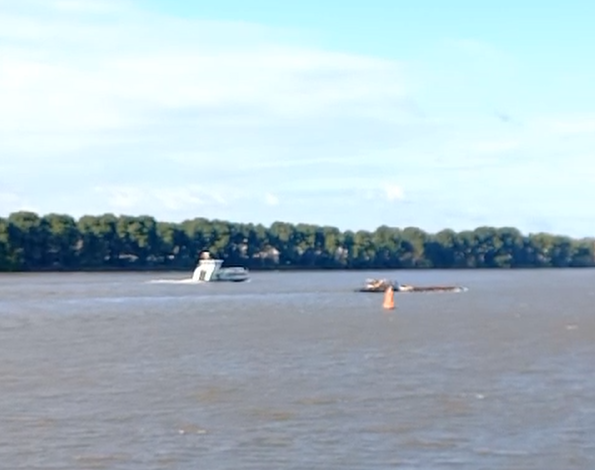
\includegraphics[width=\linewidth]{images/Evaluation/shiptrack_cut_not_analyzed.png}
			\caption{Frame aus Testdatensatz Schiffstracking}
		\end{subfigure} \hfill
		\begin{subfigure}[b]{0.45\textwidth}
			\centering
			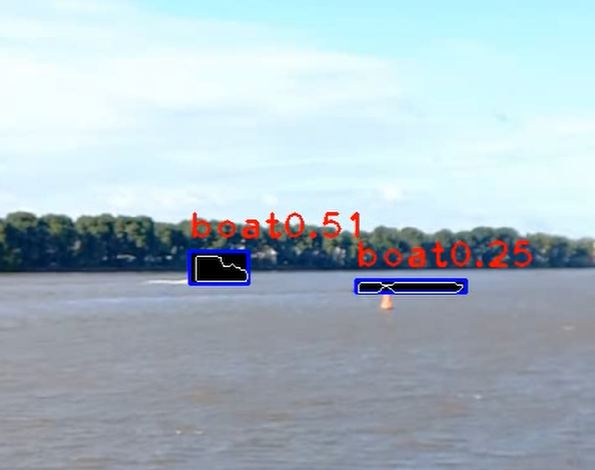
\includegraphics[width=\linewidth]{images/Evaluation/shiptrack_cut_analyzed.png}
			\caption{analysierter Testdatensatz Schiffstracking}
		\end{subfigure}
		\caption[Screenshots zu Testdatensatz Schiffstracking]{Screenshots zu Testdatensatz Schiffstracking. (a) zeigt die Testdaten ohne Bearbeitung; (b) zeigt den Frame mit YOLO analysiert und von der DCE vereinfacht (Quelle: eigene Darstellung)}
		\label{Scr:Testdatensatz_Shiptracking}
	\end{figure} 
	Die Ergebnisse der statistischen Auswertung (s. Tabelle \ref{tab:Shiptracking_Analysis}) zeigen steigende Werte in fast allen Bereichen. Die Anzahl der Punkte vor und nach DCE steigt um das ca. 26-fache im Vergleich zwischen den Videolängen an. Die Anzahl der verglichenen Winkel steigt um mehr als das 200-fache, während die Gesamtwinkelsumme wieder um den Faktor 26  ansteigt. Die Zahl der erkannten Polygone steigt hingegen nicht so stark an (ca. Faktor 22), wie die Zahl der verglichenen Polygone (ca. Faktor 25). \\
	Bei der Prozessierungszeit ist eine Steigerung um den Faktor 22 zu erkennen, während YOLO den größten Teil davon mit 31,51 Sekunden bei dem 1-sekündigem Testdatensatz, bzw. 706,76 Sekunden (11,33 Minuten) bei dem 21-sekündigem Testdatensatz ausmacht. Die DCE hat mit 0,15 Millisekunden (bzw. 19,62 Millisekunden) einen sehr geringen Anteil an der Laufzeit bei diesen Testdatensätzen, jedoch ist hier der Faktor für den Anstieg zwischen den Videos mit ca. 130 sehr hoch. \\
	Bei der SSM ist der absolute Anstieg zwischen den Videos bemerkenswert, da dieser von ca. 2 auf ca. 150 wächst und damit ungefähr um den Faktor 80 ansteigt. Der SSM pro Frame und Klasse Boot sinkt hingegen, während die Anzahl erkannter Boote massiv um den Faktor 12 (von 46 auf 1212 detektierten Booten auf allen Frames) ansteigt. Letzteres ist auch bei der Zahl der erkannten Boote pro Frame zu erkennen. \\

	\begin{table}[]
		\centering
		\caption[Auswertung Schiffstracking Datensatz]{Auswertung Schiffstracking Datensatz; S1s ist der 1-sekündige Datensatz, S21s ist der 21-sekündige Datensatz (Quelle: eigene Darstellung; Listings \ref{cd:listing_A1s_RV_shiptracking_results.txt(Y8x)}, \ref{cd:listing_A21s_RV_shiptracking_results.txt(Y8x)})}
		\label{tab:Shiptracking_Analysis}
		\begin{tabular}{l|l|l|l}
			& \textbf{S1s\_Y8x} & \textbf{S21s\_Y8x} & \textbf{Faktor} \\ \hline
		   \textit{\begin{tabular}[c]{@{}l@{}}Anzahl Punkte/Winkel\\ vor DCE\end{tabular}} & 763 & 22.093 & 28,96 \\ \hline
		   \textit{\begin{tabular}[c]{@{}l@{}}Anzahl Punkte/Winkel\\ nach DCE\end{tabular}} & 762 & 19.874 & 26,08 \\ \hline
		   \textit{\begin{tabular}[c]{@{}l@{}}Anzahl vergl. Winkel\\ bei SSM Berechnung\end{tabular}} & 1.380 & 286.468 & 207,59 \\ \hline
			&  &  &  \\ \hline
		   \textit{Gesamtwinkelsumme} & 2.392,73 & 62.363,07 & 26,06 \\ \hline
		   \textit{erk. Polygone} & 60 & 1.310 & 21,83 \\ \hline
		   \textit{vergl. Polygone} & 49 & 1.213 & 24,76 \\ \hline
			&  &  &  \\ \hline
		   \textit{\begin{tabular}[c]{@{}l@{}}Prozessierungszeit \\ (in Sek.)\end{tabular}} & 31,51 & \begin{tabular}[c]{@{}l@{}}706,76\\ (11,78 Min.)\end{tabular} & 22,79 \\ \hline
		   \textit{Dauer YOLO (in Sek.)} & 34,51 & \begin{tabular}[c]{@{}l@{}}679,66\\ (11,33 Min.)\end{tabular} & 19,69 \\ \hline
		   \textit{Dauer DCE (in ms.)} & 0,15 & 19,62 & 129,46 \\ \hline
			&  &  &  \\ \hline
		   \textit{Absolute SSM Boot} & 1,9636 & 151,1244 & 79,96 \\ \hline
		   \textit{SSM pro Fr. und Kl. Boot} & 0,0655 & 0,2354 & 3,59 \\ \hline
		   \textit{SSM pro detektierten Boot} & 0,427 & 0,1246 & 0,27 \\ \hline
		   \textit{\begin{tabular}[c]{@{}l@{}}absolute Anz. detektierter\\ Boote (in Klam. pro Fr.)\end{tabular}} & \begin{tabular}[c]{@{}l@{}}46\\ (1,53)\end{tabular} & \begin{tabular}[c]{@{}l@{}}1212\\ (1,89)\end{tabular} & \begin{tabular}[c]{@{}l@{}}12,35\\ (1,24)\end{tabular}
		   \end{tabular}
		\end{table}

	
}
%\clearpage
\subsection{Geringe und hohe DCE Substitution} 
	{Bei diesen Testdaten werden die Fälle betrachtet, bei denen DCE geringere und höhere Punktgrenzen beachten muss. Als Referenz wird der 8x Datensatz in der Länge 1 Sekunde und in der Länge 10 Sekunden genutzt. Es wird immer die RV Version der Implementierung mit dem YOLOv8x Modell betrachtet. Die DCE Grenzen sind in Tabelle \ref{tab:YOLO8_minor_more_DCE_Limits} aufgelistet. Der SSM wird aufgrund von nur kleineren Unterschieden bei den anderen Klassen anhand der beiden Hauptklassen Auto und LKW beurteilt. \\
	Im Folgenden wird sich auf den 10-sekündigen Testdatensatz bezogen, da die Ergebnisse auf den 1-sekündigen Datensatz übertragbar sind. Hier ist die einzige Besonderheit das alle Werte deutlich geringer sind (s. Tabelle \ref{tab:YOLO8_minor_more_DCE_A1s}, S. \pageref{tab:YOLO8_minor_more_DCE_A1s}  und Tabelle \ref{tab:Minor_More_DCE_SSMs_A1s}, S. \pageref{tab:Minor_More_DCE_SSMs_A1s}). \\
	\begin{table}[ht]
		\caption[Einstellungen der verschiedenen DCE Substitutionslimits]{Einstellungen der verschiedenen DCE Substitutionslimits (Quelle: eigene Darstellung; Listings \ref{cd:listing_A1s_RV_minor_results.txt(Y8x)}, \ref{cd:listing_A1s_RV_more_results.txt(Y8x)}, \ref{cd:listing_A10s_RV_minor_results.txt(Y8x)}, \ref{cd:listing_A10s_RV_more_results.txt(Y8x)})}
		\label{tab:YOLO8_minor_more_DCE_Limits}
		\centering
		\begin{tabular}{l|l|l|l}
		 & \textbf{\begin{tabular}[c]{@{}l@{}}geringe DCE\\ Punktgrenzen\end{tabular}} & \textbf{Referenz} & \textbf{\begin{tabular}[c]{@{}l@{}}hohe DCE\\ Punktgrenzen\end{tabular}} \\ \hline
		\textit{Kl. Auto} & 5 & 8 & 60 \\ \hline
		\textit{Kl. Motorrad} & 3 & 5 & 25 \\ \hline
		\textit{Kl. LKW} & 6 & 11 & 40 \\ \hline
		\textit{anderes Objekt} & 5 & 20 & 100
		\end{tabular}
		\end{table} In Tabelle \ref{tab:YOLO8_minor_more_DCE_A10s} ist zu sehen, dass die Punktanzahl vor der DCE Vereinfachung bei allen drei Testdurchläufen exakt gleich gewesen ist. Ein Unterschied ist bei der Anzahl der Punkte nach dem Durchlauf der DCE zu erkennen, da bei der geringen Punktgrenze ein niedriger Wert und bei der hohen Punktgrenze ein höherer Wert als beim Referenzdatensatz gemessen wurde. Die Anzahl der verglichenen Winkel steigt im Vergleich zwischen allen drei Durchläufen stark an. \\
		Dieser starke Anstieg ist auch bei der Gesamtwinkelsumme zu erkennen. Die erkannten und verglichenen Polygone bleiben hingegen über alle 3 Testdurchläufe exakt gleich. \\
		Wenn man die Dauer der Prozessierung betrachtet, ist eine geringe Verbesserung zu einer kürzeren Dauer zu erkennen.\\
			\begin{table}[ht]
				\caption[Vergleich der Basisdaten beim 10-sekündigem Video (300 Frames) und verschiedenen DCE Substitutionslimits]{Vergleich der Basisdaten bei 10-sekündigem Video (300 Frames) und verschiedenen DCE Substitutionslimits (Quelle: eigene Darstellung; Listings \ref{cd:listing_A10s_RV_minor_results.txt(Y8x)}, \ref{cd:listing_A10s_RV_more_results.txt(Y8x)})}
				\label{tab:YOLO8_minor_more_DCE_A10s}
				\centering
				\begin{tabular}{l|l|l|l}
					& \textbf{\begin{tabular}[c]{@{}l@{}}geringe DCE\\ Punktgrenzen\end{tabular}} & \textbf{Referenz} & \textbf{\begin{tabular}[c]{@{}l@{}}hohe DCE\\ Punktgrenzen\end{tabular}} \\ \hline
				   \textit{\begin{tabular}[c]{@{}l@{}}Anzahl Punkte/Winkel \\ vor DCE\end{tabular}} & 57.673 & 57.673 & 57.673 \\ \hline
				   \textit{\begin{tabular}[c]{@{}l@{}}Anzahl Punkte/Winkel\\ nach DCE\end{tabular}} & 11.584 & 20.132 & 43.040 \\ \hline
				   \textit{\begin{tabular}[c]{@{}l@{}}Anzahl vergl. Winkel\\ bei SSM Berechnung\end{tabular}} & 39.703 & 119.714 & 769.311 \\ \hline
				   \textit{} &  &  &  \\ \hline
				   \textit{Gesamtwinkelsumme} & 36.389,37 & 63.172,79 & 135.064,50 \\ \hline
				   \textit{erkannte Polygone} & 2.104 & 2.104 & 2.104 \\ \hline
				   \textit{verglichene Polygone} & 1.960 & 1.960 & 1.960 \\ \hline
				   \textit{Prozessierungszeit (in Min.)} & 8,48 & 7,99 & 7,22
				   \end{tabular}
				\end{table}Bei der SSM von den Klassen Auto und LKW (s. Tabelle \ref{tab:Minor_More_DCE_SSMs_A10s}) sind ähnliche Effekte zu sehen. Die absolute Abweichung bei der Klasse Auto, wie auch bei der Klasse LKW steigt um mehr als das Doppelte im Vergleich von dem geringen zum hohen DCE Substitionslimit. Den gleichen Effekt kann man auch der SSM pro Frame und Klasse Auto oder LKW und bei der SSM pro detektiertem Auto oder LKW sehen. Die absolute Anzahl Auto und LKW (auch pro Frame) bleibt hingegen über alle drei Testfälle exakt gleich.	
				\begin{table}[ht]
					\caption[Vergleich der SSMs bei verschiedenen DCE Substitionslimits bei einem 10-sekündigem Video (300 Frames) ]{Vergleich der SSMs bei verschiedenen DCE Substitionslimits bei einem 10-sekündigem Video (300 Frames) (Quelle: eigene Darstellung; Listings \ref{cd:listing_A10s_RV_minor_results.txt(Y8x)}, \ref{cd:listing_A10s_RV_more_results.txt(Y8x)})}
					\label{tab:Minor_More_DCE_SSMs_A10s}
					\centering
					\begin{tabular}{l|l|l|l}
						& \textbf{\begin{tabular}[c]{@{}l@{}}geringe DCE\\ Punktgrenzen\end{tabular}} & \textbf{Referenz} & \textbf{\begin{tabular}[c]{@{}l@{}}hohe DCE\\ Punktgrenzen\end{tabular}} \\ \hline
					   \textit{Absolute SSM Auto} & 43,438 & 58,6721 & 97,1323 \\ \hline
					   \textit{SSM pro Fr. und Kl. Auto} & 0,1448 & 0,1956 & 0,3238 \\ \hline
					   \textit{SSM pro detektiertes Auto} & 0,0827 & 0,1118 & 0,1850 \\ \hline
					   \textit{\begin{tabular}[c]{@{}l@{}}absolute Anz. detektierter\\ Autos (in Kl. pr. Fr.)\end{tabular}} & \begin{tabular}[c]{@{}l@{}}525\\ (1,75)\end{tabular} & \begin{tabular}[c]{@{}l@{}}525\\ (1,75)\end{tabular} & \begin{tabular}[c]{@{}l@{}}525\\ (1,75)\end{tabular} \\ \hline
					   \textit{} &  &  &  \\ \hline
					   \textit{Absolute SSM LKW} & 112,7181 & 154,3962 & 255,6707 \\ \hline
					   \textit{SSM pro Fr. und Kl. LKW} & 0,3757 & 0,5147 & 0,8522 \\ \hline
					   \textit{SSM pro detektierten LKW} & 0,1553 & 0,2127 & 0,3522 \\ \hline
					   \textit{\begin{tabular}[c]{@{}l@{}}Absolute Anz. detektierter\\ LKW (in Kl. pro Fr.)\end{tabular}} & \begin{tabular}[c]{@{}l@{}}726\\ (2,42)\end{tabular} & \begin{tabular}[c]{@{}l@{}}726\\ (2,42)\end{tabular} & \begin{tabular}[c]{@{}l@{}}726\\ (2,42)\end{tabular}
					   \end{tabular}
					\end{table}
		
	}
%\clearpage
\subsection{Gleiche DCE Substitionslimits}{
	Bei diesem Testfall wurden gleiche DCE Substitionslimits (s. Tabelle \ref{tab:YOLO8_sameDCELimits_overview}) für alle Objekte in den Einstellungen vermerkt. Alle anderen Einstellungen wurden aus den Standardtestfällen übernommen, außer das das Video nicht vollständig schwarz gerendert wurde, sondern nur die Boundingboxen der detektierten Objekte durch schwarze Pixel gefüllt wurden. Der SSM wird aufgrund von nur kleineren Unterschieden bei den anderen Klassen anhand der beiden Hauptklassen Auto und LKW beurteilt. \\
	\begin{table}[ht]
		\centering
		\caption[Vergleich der Basisdaten bei 10-sekündigem Video (300 Frames) und verschiedenen gleichen DCE Substitutionslimits]{Vergleich der Basisdaten bei 10-sekündigem Video (300 Frames) und verschiedenen gleichen DCE Substitutionslimits (Quelle: eigene Darstellung; Listings \ref{cd:listing_A10s_RV_minorSame_results.txt(Y8x)}; \ref{cd:listing_A10s_RV_results.txt(Y8x)}; \ref{cd:listing_A10s_RV_moreSame_results.txt(Y8x)})}
		\label{tab:YOLO8_sameDCELimits_basicdata}
		\begin{tabular}{l|l|l|l}
		 & \textbf{\begin{tabular}[c]{@{}l@{}}geringe gleiche \\ Limits\end{tabular}} & \textbf{\begin{tabular}[c]{@{}l@{}}Referenz \\ (10 Sek. Video)\end{tabular}} & \textbf{\begin{tabular}[c]{@{}l@{}}hohe gleiche \\ Limits\end{tabular}} \\ \hline
		\textit{\begin{tabular}[c]{@{}l@{}}Anzahl Punkte/Winkel \\ vor DCE\end{tabular}} & 57.673 & 57.673 & 57.673 \\ \hline
		\textit{\begin{tabular}[c]{@{}l@{}}Anzahl Punkte/Winkel\\ nach DCE\end{tabular}} & 21.540 & 20.132 & 30.611 \\ \hline
		\textit{\begin{tabular}[c]{@{}l@{}}Anzahl vergl. Winkel\\ bei SSM Berechnung\end{tabular}} & 135.024 & 119.714 & 307.261 \\ \hline
		\textit{} &  &  &  \\ \hline
		\textit{Gesamtwinkelsumme} & 67.586,21 & 63.172,79 & 96.037,00 \\ \hline
		\textit{erkannte Polygone} & 2.104 & 2.104 & 2.104 \\ \hline
		\textit{verglichene Polygone} & 1.960 & 1.960 & 1.960 \\ \hline
		\textit{Prozessierungszeit (in Min.)} & 8,28 & 7,99 & 8,07
		\end{tabular}
	\end{table}

	Die Anzahl der detektierten Punkte vor DCE entspricht von beiden Testdurchläufen exakt der Differenz und ist damit exakt auch zueinander gleich. Bei der Anzahl von Punkten nach der DCE ist die Zahl bei geringen gleichen Limits minimal höher als bei der Referenz, während bei hohen Limits die Zahl stark ansteigt. Die Zahl der verglichenen Winkel bei der SSM Berechnung ist bei geringen gleichen Limits höher als bei dem Referenzdatensatz und bei hohen gleichen Limits steigt diese Zahl sehr stark an. Ähnliche Phänomene sind bei der Gesamtwinkelsumme zu sehen. Die Zahl der erkannten und verglichenen Polygone bleibt bei allen drei Videos gleich. \\
	Bei der Prozessierungszeit ist eine etwas längere Dauer bei geringen gleichen Limits zu erkennen, während bei hohen gleichen Limits die Dauer fast gleich bleibt.
	\begin{table}[]
		\centering
		\caption[Vergleich der SSM bei 10-sekündigem Video (300 Frames) und verschiedenen gleichen DCE Substitutionslimits]{Vergleich der SSM bei 10-sekündigem Video (300 Frames) und verschiedenen gleichen DCE Substitutionslimits (Quelle: eigene Darstellung; Listings \ref{cd:listing_A10s_RV_minorSame_results.txt(Y8x)}; \ref{cd:listing_A10s_RV_results.txt(Y8x)}; \ref{cd:listing_A10s_RV_moreSame_results.txt(Y8x)})}
		\label{tab:YOLO8_SameDCESubst_A10s_SSM}
		\begin{tabular}{l|l|l|l}
			& \textbf{\begin{tabular}[c]{@{}l@{}}geringe gleiche\\ Limits\end{tabular}} & \textbf{\begin{tabular}[c]{@{}l@{}}Referenz\\ (10 Sek. Video)\end{tabular}} & \textbf{\begin{tabular}[c]{@{}l@{}}hohe gleiche\\ Limits\end{tabular}} \\ \hline
		\textit{Absolute SSM Auto} & 67,2633 & 58,6721 & 83,1752 \\ \hline
		\textit{SSM pro Fr. und Kl. Auto} & 0,2242 & 0,1956 & 0,2773 \\ \hline
		\textit{SSM pro detektiertes Auto} & 0,1281 & 0,1118 & 0,1584 \\ \hline
		\textit{\begin{tabular}[c]{@{}l@{}}absolute Anz. detektierter\\ Autos (in Kl. pr. Fr.)\end{tabular}} & \begin{tabular}[c]{@{}l@{}}525\\ (1,75)\end{tabular} & \begin{tabular}[c]{@{}l@{}}525\\ (1,75)\end{tabular} & \begin{tabular}[c]{@{}l@{}}525\\ (1,75)\end{tabular} \\ \hline
		\textit{} &  &  &  \\ \hline
		\textit{Absolute SSM LKW} & 154,3962 & 154,3962 & 212,9169 \\ \hline
		\textit{SSM pro Fr. und Kl. LKW} & 0,5147 & 0,5147 & 0,7097 \\ \hline
		\textit{SSM pro detektierten LKW} & 0,2127 & 0,2127 & 0,2933 \\ \hline
		\textit{\begin{tabular}[c]{@{}l@{}}Absolute Anz. detektierter\\ LKW (in Kl. pro Fr.)\end{tabular}} & \begin{tabular}[c]{@{}l@{}}726\\ (2,42)\end{tabular} & \begin{tabular}[c]{@{}l@{}}726\\ (2,42)\end{tabular} & \begin{tabular}[c]{@{}l@{}}726\\ (2,42)\end{tabular}
		\end{tabular}
	\end{table}

	Bei SSM ist für die Klasse Autos zu erkennen, dass die absolute Zahl bei geringen gleichen Limits im Vergleich zur Referenz ansteigt. In größerem Maße ist dies auch bei den hohen gleichen Limits vorhanden. Bei der SSM pro Frame und Klasse Auto und bei der SSM pro detektiertes Auto ist dieser Effekt ebenfalls erkennbar, während die absolute Anzahl detektierter Autos konstant bleibt. \\
	Bei der absoluten SSM pro LKW ist zwischen der Referenz und den geringen gleichen Limits kein Unterschied vorhanden. Ein Unterschied zu den hohen gleichen Limits ist hingegen mit einer Steigerung der absoluten SSM mit einem kleinen Anstieg der SSM pro Frame und Klasse LKW, bzw. pro detektiertem LKW, zu sehen. Die absolute Anzahl detektierte LKW und die Zahl der LKW pro Frame bleibt, wie bei der Klasse Autos, über alle Videos konstant. 

	\begin{table}[]
		\centering
		\caption[DCE Substitutionslimits bei gleichen Limits für alle Klassen]{DCE Substitutionslimits bei gleichen Limits für alle Klassen (Quelle: eigene Darstellung; Listings \ref{cd:listing_A10s_RV_minorSame_results.txt(Y8x)}; \ref{cd:listing_A10s_RV_results.txt(Y8x)}; \ref{cd:listing_A10s_RV_moreSame_results.txt(Y8x)})}
		\label{tab:YOLO8_sameDCELimits_overview}
		\begin{tabular}{l|l|l|l}
			& \textbf{\begin{tabular}[c]{@{}l@{}}geringe gleiche\\ Limits\end{tabular}} & \textbf{Referenz} & \textbf{\begin{tabular}[c]{@{}l@{}}hohe gleiche\\ Limits\end{tabular}} \\ \hline
		\textit{Kl. Auto} & 11 & 8 & 20 \\ \hline
		\textit{KL. Motorrad} & 11 & 5 & 20 \\ \hline
		\textit{Kl. LKW} & 11 & 11 & 20 \\ \hline
		\textit{anderes Objekt} & 11 & 20 & 20
		\end{tabular}
	\end{table}
		
}	
%\clearpage
\subsection{Langer Testdatensatz}{


\begin{table}[h]
	\centering
	\caption[Vergleich der Basisdaten bei 30-sekündigem Video (900 Frames)]{Vergleich der Basisdaten bei 30-sekündigem Video (900 Frames) (Quelle: eigene Darstellung; Listings \ref{cd:listing_A1s_RV_results.txt(Y8x)}; \ref{cd:listing_A10s_RV_results.txt(Y8x)}; \ref{cd:listing_A30s_RV_results.txt(Y8x)})}
	\label{tab:YOLO8_longshot_A30s_basicdata}
	\begin{tabular}{l|l|l|l}
	 & \textbf{\begin{tabular}[c]{@{}l@{}}Referenz\\ (1 Sek. Video)\end{tabular}} & \textbf{\begin{tabular}[c]{@{}l@{}}Referenz \\ (10 Sek. Video)\end{tabular}} & \textbf{30 Sek. Video} \\ \hline
	\textit{\begin{tabular}[c]{@{}l@{}}Anzahl Punkte/Winkel \\ vor DCE\end{tabular}} & 5.325 & 57.673 & 193.384 \\ \hline
	\textit{\begin{tabular}[c]{@{}l@{}}Anzahl Punkte/Winkel\\ nach DCE\end{tabular}} & 1.988 & 20.132 & 66.931 \\ \hline
	\textit{\begin{tabular}[c]{@{}l@{}}Anzahl vergl. Winkel\\ bei SSM Berechnung\end{tabular}} & 44.858 & 119.714 & 407.057 \\ \hline
	\textit{} &  &  &  \\ \hline
	\textit{Gesamtwinkelsumme} & 6.237,21 & 63.172,79 & 210.030,73 \\ \hline
	\textit{erkannte Polygone} & 214 & 2.104 & 6.877 \\ \hline
	\textit{verglichene Polygone} & 194 & 1.960 & 6.492 \\ \hline
	\textit{Prozessierungszeit (in Min.)} & 0,73 & 7,99 & 27,32
	\end{tabular}
	\end{table}

	Bei diesem Testfall wurde ein längerer Testdatensatz von 30 Sekunden, bzw. 900 Frames, durch die DCE vereinfacht. Es wurden die gleichen Einstellungen, wie bei den Standardtestfällen eingesetzt, außer das das Video nicht vollständig schwarz gerendert wurde, sondern nur die Boundingboxen der detektierten Objekte durch schwarze Pixel gefüllt wurden. Als Referenzvideos sind in den Tabellen \ref{tab:YOLO8_longshot_A30s_basicdata} und \ref{tab:YOLO8_longshots_SSM} die Datensätze mit jeweils der Dauer 1 Sekunde (30 Frames) und 10 Sekunden (300 Frames) aufgeführt. Der SSM wird aufgrund von nur kleineren Unterschieden bei den anderen Klassen anhand der beiden Hauptklassen Auto und LKW beurteilt. \\
	Bei Tabelle \ref{tab:YOLO8_longshot_A30s_basicdata} ist zu erkennen, dass die Anzahl der detektierten Punkte sich zwischen den beiden Referenzdaten um den Faktor 10 erhöht und bei dem 30-sekündigem Datensatz der Faktor ungefähr 3 beträgt, wenn man ihn mit der 10-sekündigen Referenz vergleicht. Ähnliche Steigerungsfaktoren kann man auch bei der Anzahl der Punkte nach der Vereinfachung durch DCE zwischen allen drei Videos erkennen. Bei der Anzahl der verglichenen Winkel ist wiederum ein deutlich höhere Anstieg zu erkennen, während bei der Gesamtwinkelsumme, der Anzahl der erkannten und den verglichenen Polygone wieder ungefähr die gleichen Faktoren, wie bei der Gesamtpunktanzahl vor und nach DCE angewendet werden können. \\
	Bei der Prozessierungszeit ist jedoch ein deutlicher Anstieg bei dem 30-sekündigen Testdatensatz zu sehen, der jedoch auch recht linear verläuft.

	
	

		\begin{table}[h]
			\centering
			\caption[Vergleich der SSM bei 30-sekündigem Video (900 Frames)]{Vergleich der SSM bei 30-sekündigem Video (900 Frames) (Quelle: eigene Darstellung; Listings \ref{cd:listing_A1s_RV_results.txt(Y8x)}; \ref{cd:listing_A10s_RV_results.txt(Y8x)}; \ref{cd:listing_A30s_RV_results.txt(Y8x)}) }
			\label{tab:YOLO8_longshots_SSM}
			\begin{tabular}{l|l|l|l}
			 & \textbf{\begin{tabular}[c]{@{}l@{}}Referenz\\ (1 Sek. Video)\end{tabular}} & \textbf{\begin{tabular}[c]{@{}l@{}}Referenz\\ (10 Sek. Video)\end{tabular}} & \textbf{30 Sek. Video} \\ \hline
			\textit{Absolute SSM Auto} & 4,1018 & 58,6721 & 161,3262 \\ \hline
			\textit{SSM pro Fr. und Kl. Auto} & 0,1367 & 0,1956 & 0,1793 \\ \hline
			\textit{SSM pro detektiertes Auto} & 0,0672 & 0,1118 & 0,1014 \\ \hline
			\textit{\begin{tabular}[c]{@{}l@{}}absolute Anz. detektierter\\ Autos (in Kl. pr. Fr.)\end{tabular}} & \begin{tabular}[c]{@{}l@{}}60\\ (2,03)\end{tabular} & \begin{tabular}[c]{@{}l@{}}525\\ (1,75)\end{tabular} & \begin{tabular}[c]{@{}l@{}}1.591\\ (1,77)\end{tabular} \\ \hline
			\textit{} &  &  &  \\ \hline
			\textit{Absolute SSM LKW} & 11,8367 & 154,3962 & 540,7660 \\ \hline
			\textit{SSM pro Fr. und Kl. LKW} & 0,3946 & 0,5147 & 0,6009 \\ \hline
			\textit{SSM pro detektierten LKW} & 0,1767 & 0,2127 & 0,2120 \\ \hline
			\textit{\begin{tabular}[c]{@{}l@{}}Absolute Anz. detektierter\\ LKW (in Kl. pro Fr.)\end{tabular}} & \begin{tabular}[c]{@{}l@{}}67\\ (2,23)\end{tabular} & \begin{tabular}[c]{@{}l@{}}726\\ (2,42)\end{tabular} & \begin{tabular}[c]{@{}l@{}}2.551\\ (2,83)\end{tabular}
			\end{tabular}
			\end{table}
	Bei der absoluten SSM der Klasse Auto sind ähnliche Steigerungsfakoren, wie bei der Punktanzahl vor und nach DCE zu vorhanden (s. Tabelle \ref{tab:YOLO8_longshots_SSM}). Die SSM pro Frame und Klasse Auto, bzw. LKW, steigt hingegen minimal bei dem 10-sekündigen Testdatensatz an, während die SSM bei dem 30-sekündigen Testdatensatz marginal absinkt. Dies ist auch bei der SSM pro detektiertem Auto und LKW zu erkennen. Die absolute Anzahl detektierter Autos und LKW steigt mit der Länge des Testdatensatzes an. Jedoch sinkt die Anzahl detektierter Autos pro Frame, während die Anzahl detektierter LKW pro Frame ansteigt.\\
	

		
	
}




\cleardoubleoddemptypage


%!TEX root = ../thesis.tex
\chapter{Diskussion}
\label{ch:Diskussion}
{ \todo{überarbeiten alles}
	Die beiden verschiedenen YOLO Implementierungen in der EF und RV Version sind sehr ähnlich im Ergebnis und Aufbau. Es zeigt sich jedoch in der Evaluation , dass die EF Variante länger für die Berechnung benötigt und damit ineffektiver ist (siehe Kap. \ref{sec:Ergebnisse}). Dies liegt daran, dass die EF Variante das Video erst in einzelne Frames zerlegt und erst dann YOLO anwendet. Dadurch ist die Prozessierung mit YOLO ineffektiver aber möglicherweise ressourcenschonender im RAM Verbrauch. \todo{das muss überprüft werden; muss mal in die längeren Evaluationsvideos gucken, wie da die Basisdaten ist} Das Zusammensetzen der einzelnen analysierten Frames zu einem Video verlängert die Prozessierungszeit zusätzlich, dies geschieht jedoch auch in der RV Version. \\
	Die RV Version besitzt den Vorteil, dass durch die direkte Verarbeitung des Videos mit dem sehr effiziente geschriebenen YOLO Algorithmus alle Prozessorkerne mitsamt der Grafikkarte vollständig ausgelastet werden können. Zusätzlich steigt jedoch der RAM Verbrauch stark an, da YOLO dort jedes Frame speichert und analysiert. Dies sorgt für eine Zeitersparnis beim Programm. \\ 
	Die DCE Implementierung ist relativ ineffizient, da der K Wert für jeden Punkt im Polygon neu berechnet werden muss, nachdem ein Punkt entfernt wurde. Dies könnte optimiert werden, indem mehrere Punkte eines Polygons gleichzeitig während einer DCE Iteration entfernt werden. Weitere Möglichkeiten wären effizientere Schleifenstrukturen oder Multithreading bei der Berechnung des K Wertes. \\
	Es ist außerdem zu erkennen, dass unterschiedliche YOLO Modelle nur geringe Auswirkungen auf die Gesamtlaufzeit des Programmes haben. Die DCE hat deutlich höheren Einfluss. \\
	
	Mit einem besseren YOLO Modell steigt die SSM für jede Klasse pro Polygon an, weil die Anzahl der erkannten Objekte steigt. Dies kann durch die größeren Trainingsdaten erklärt werden. Die steigende Abweichung, beispielsweise von ca. 20 über ca. 90. bis zu ca. 114 Grad pro detektiertes Auto kann mit der unterschiedlichen Vereinfachung der DCE begründen. Ein Auto ist im ersten Frame anders vereinfacht worden, als im nächsten Frame, wo möglicherweise andere Punkte zum Polygon hinzugekommen sind oder entfernt wurden. Diese Vereinfachung kann für jedes Polygon anders verlaufen, da die DCE die Relevanz von jedem Punkt in jedem neuen Polygon neu berechnet und YOLO die Umrisse mit kleineren Abweichungen ausgibt.

	Bei Objekten, die bei der DCE Vereinfachung als \glqq other Object\grqq{} behandelt werden, können die deutlich höheren SSMs durch die deutlich höheren Punktzahlen, auf die die DCE am Ende reduziert, erklärt werden. Diese führt zu einer steigenden Gesamtwinkelsumme pro Polygon, welches auch zu einer höheren Abweichung der Gesamtwinkelsumme im nächsten Frame führt. Dies kann die gleichen Ursachen wie im obigen Abschnitt haben und ist inbesondere in Kap. \ref{ev:shiptracking} zu erkennen. \\
	
	Einen Einfluss auf absolute Anzahl von Autos können LKW, die Autos transportieren, haben. Einer dieser Autotransporter ist im Testdatensatz zu sehen, was zu einer Erhöhung der absoluten Anzahl von Autos führt, als dieser teilweise aus dem Bild fährt, wodurch nur noch die auf dem Anhänger stehenden Autos von YOLO detektiert werden. Weitere falsche Detektierungen können durch Schilder und andere Objekte verursacht werden. \\

	Wenn man die Ergebnisse aus der Sicht der exakten Berechnungsmöglichkeiten heutiger Computer beurteilt, müsste die Abweichung aus gegen 0 konvergierende Werten bestehen. Durch die hohen Punktunterschiede zwischen den einzelnen Klassen und nicht exaktes Umriss- und Klassifizierungstracking von YOLO ist der leichte Anstieg der SSM erklärbar. Das Tracking von YOLO wechselt zwischen der am besten passenden Klassifizierung, obwohl das Objekt intuitiv vom Betrachter beurteilt auch weiterhin der wirklichen, real übereinstimmenden vorher erkannten Klasse entspricht. 

	\begin{itemize}
		\item warum kann man das alles nicht direkt mit YOLO machen? Rechenleistung ist doch eigentlich genug vorhanden (auch auf Drohnen bzw. Wildkameras)
	\end{itemize}

	\section{Einordnung der Evaluationsergebnisse}
	{
		Bei den allgemeinen Daten, die der Evaluation (s. Kap. \ref{subsec:allgErkenntis}) beschrieben wurden, ist zu erkennen, dass die Zahl der Punkte vor DCE minimal steigt, da auch die Zahl der Polygone ansteigt (s. Tabelle \ref{tab:YOLO8_A10s}). Dies kann daran liegen, dass bei den größeren YOLO Modellen die Detektion und Klassifizierung von Objekten genauer und häufiger erfolgt. Die steigende Punktanzahl nach der DCE Vereinfachung kann ebenfalls mit den größeren YOLO Modellen erklärt werden, da diese auch zu einer höheren Zahl von erkannten Polygonen führen. Aus diesem Grund korreliert die Zahl der Punkte nach der DCE Vereinfachung mit der Zahl der erkannten Polygone (bzw. detektierter Objekte).\\
		Die Anzahl der Punkte nach der DCE Vereinfachung bleibt relativ konstant zwischen den Modellen 8m und 8x, da 8m recht zuverlässig alle Objekte im Video detektiert. Dadurch, dass diese Objekte als Polygone danach von der DCE vereinfacht werden, bleibt die Anzahl der Punkte nach der DCE Vereinfachung recht konstant. Die Anzahl der verglichenen Winkel steigt hingegen deutlich schneller an als die Punktanzahl, da die Polygone permutiert werden. \\
		Bei der SSM ist zu sehen, dass die Zahl der Polygone von 8n zu 8m stark ansteigt, weil mehr Objekte detektiert werden. Im Vergleich von 8m zu 8x bleibt die Zahl der Polygone relativ  konstant, weil beide Modelle alle Objekte detektieren, bzw. die Steigerung zwischen 8m und 8x ist sehr gering, weil im Testdatensatz selbst nicht mehr Objekte enthalten sind. \\
		Die Laufzeit des Programmes unterscheidet sich zwischen den Implementierungen, da YOLO bei direkter Verarbeitung den Vorteil der effizienten Implementierung und vollständigen CPU Auslastung nutzen kann. Die EV Version ist ineffektiv implementiert, weil YOLO jedes Bild einzeln analysiert; das Programm auf dieses Einzelbild DCE anwendet und wieder mit dem nächsten Frame von vorne anfängt. Dieser Unterschied ist insbesondere bei der Verwendung der besser trainierten YOLO Modelle zu erkennen, da dort die Analyse mit YOLO mehr Zeit und Ressourcen benötigt. \\
		Außerdem ist auffällig, dass in den Testdatensätzen Züge detektiert werden. Diese Fehldetektion von LKW kann mit besseren Modellen stark verringert und nahezu eliminiert werden, wie auch in Tabelle \ref{tab:YOLO8_A10s_SSM} zu sehen. Die Anzahl der detektierten Züge entspricht ungefähr der Anzahl der im nächsthöheren Modell mehr detektierten LKW. \\

		Wenn man nun die SSM beurteilt, ist zu erkennen, dass die absolute SSM mit der Verwendung des größeren YOLO Modell steigt, weil mehr Objekte der jeweiligen Klasse richtig detektiert und erkannt werden. Da die SSM pro Frame und Klasse direkt von dem Absolutwert abhängt und weniger Falschdetektionen diesen Wert verzerren, steigt dieser Wert ebenfalls bei Verwendung der besseren YOLO Modelle. Dieser Effekt ist auch bei der absoluten Anzahl detektierter Objekte (bspw. Autos) zu erkennen (s. Tab. \ref{tab:YOLO8_A10s_SSM}). \\
		Bei der Klasse LKW verdoppelt sich die absolute SSM, weil die Punktzahl, auf die DCE diese Objekte reduziert, deutlich höher ist (11) als die von der Klasse Autos (8). Da die absolute SSM steigt, wachsen auch hier die anderen Werte, wie SSM pro Frame und Klasse LKW und SSM pro detektiertem LKW. Bei der absoluten Anzahl der Klasse Zug ist hingegen die Verringerung auf 1 durch die Verwendung der besseren YOLO Modelle zu erklären, da bei 8x 1 LKW falsch detektiert wird. Außerdem wird bei 8x kein LKW als Bus mehr (falsch) detektiert. 
		Aus den obigen Gründen folgt, dass ein bessere trainiertes Modell eine bessere Erkennungsleistung bei längerer Berechnungsdauer hat.  \\

		Bei den weiteren Testfällen ist beim Schiffstracking Datensatz zu sehen, dass die Punktanzahlen vor und nach der DCE Berechnung in etwa um die Videolänge ansteigen. Auch hier ist der Anstieg der Anzahl der verglichenen Winkel bei der SSM Berechnung exponentiell aufgrund der Polygonpermutation. Der Anstieg der Prozessierungszeit entspricht ebenfalls ungefähr dem Unterschied der Sekundenzahl der Testdatensätze (1 Sekunde und 21 Sekunden, Anstiegsfaktor 22 bei Prozessierungszeit). Recht kurz ist hingegen die Berechnungszeit der DCE, die dennoch zwischen den Testdatensätzen ansteigt. Dieser Anstieg liegt an der steigenden Polygonanzahl, ist aber sehr gering, weil allgemein bei diesen Testdaten wenige Polygone vereinfacht werden müssen. \\
		Die Minderung der SSM pro Frame und Klasse Boot hängt mit der nicht so stark ansteigenden absoluten SSM im Gegensatz zur stark steigenden absoluten Anzahl detektierter Boote  zusammen. Die Anzahl der detektierten Boote steigt beim 21-sekündigen Testdatensatz aufgrund der Länge an.\\
		Aus diesem Testfall gefolgert werden, dass sich der Anwendungszweck des formbasierten Objekttrackings mit der DCE nicht nur auf den angedachten Anwendungsfall Verkehrstracking beschränkt, sondern auch andere Anwendungsfälle, wie Schiffs- oder Flugzeugtracking, möglich sind. Damit ist der in Kap. \ref{sec:Aufbau_Arbeit} genannte Grund für den Testfall erfüllt. Die einzige Einschränkung hier ist die Anzahl der Klassen, die von YOLO unterschieden werden können.\\

		Bei dem Testfall, der geringe und hohe DCE Substitionslimits abdeckt, ist Folgendes aufgefallen. Die Anzahl der Punkte vor dem DCE Durchlauf ist bei allen 3 Vergleichstestdatensätzen exakt gleich, weil das Quellvideo und das YOLO Modell übereinstimmen. Außerdem ist YOLO ein deterministischer Algorithmus, der bei gleichen Einstellungsparametern und gleichem Modell, stets das exakt gleiche Ergebnis berechnet. Dies gilt auch für die Anzahlen der erkannten und verglichenen Polygone, sowie bei der absoluten Anzahl detektierte Objekte (und dieser Anzahl der Objekte pro Frame), die aus diesen Gründen exakt gleich sind bei allen 3 Vergleichstestdatensätzen. \\
		Die Anzahl der Punkte nach der DCE Berechnung ist unterschiedlich, weil DCE durch die verschiedenen Substitionslimits auf die Polygone auf verschiedenen Punktgrenzen reduziert. Dies ist der Fall, weil durch die Reduktion der Punkte durch DCE, je nach Einstellungen, mehr oder weniger Punkte die Polygon repräsentieren. Dieser Effekt betrifft auch die Zahl der verglichenen Winkel bei der SSM Berechnung, die jedoch exponentiell wegen der Permutation ansteigt. Von der Punktanzahl nach der DCE Vereinfachung ist die Gesamtwinkelsumme ebenfalls abhängig, deshalb steigt diese stark an. \\
		Die Dauer der Prozessierung sinkt, weil der Berechnungsaufwand für die DCE Vereinfachung nicht mehr so hoch ist. \\
		Da die weiteren SSM Werte von dem absoluten SSM Wert und dieser von der Punktanzahl nach der DCE abhängig ist, sind dort ähnliche Steigerungen zu erkennen. \\
		Die absolute Anzahl detektierter Autos und LKW, bzw. die Anzahl dieser Objekte pro Frame, bleibt über alle 3 Testdatensätze gleich, weil der YOLO Algorithmus, wie oben erläutert, deterministisch ist. \\
		An diesem Testfall konnte gut erläutert werden, welche Änderungen an den Einstellungen die Ergebnisse beim Objekttracking beeinflussen. Es konnte herausgefunden werden, dass der DCE Algorithmus mit optimierten Substitionslimits eine bessere Leistung erzielt. \\


		




	}

	Evaluation Stichpunkte
	\begin{itemize}
		
		
	
		
		
		\item Gleiche DCE Substitionslimits
		\begin{itemize}
			\item Anstieg der Anzahl Punkte nach DCE bei geringen gleichen Limits ist durch das Anheben mancher Substitutionslimits im VGL zur Referenz zu erklären; erklärt auch großen Anstieg bei hohen gleichen Limits
			\item Anzahl vergl. Winkel korreliert mit Anzahl Punkte nach DCE -> Deshalb die Schwankungen bei geringen und hohen Limits im Vergleich zur Referenz
			\item gilt auch für Gesamtwinkelsumme
			\item Erkannte und verglichene Polygone bleiben gleich (gleiches Video, gleicher deterministischer Algorithmus)
			\item Prozessierungszeit bei geringen gleichen Limits steigt an, weil DCE länger rechnen muss: bei hohen gleichen Limits ebenfalls marginaler Anstieg, aber fast gleich; weil sich die Erhöhung über alle Klassen hinweg im Vergleich zur Referenz ausgleicht
			\item XXXXXXXXXXXXXXXXXXXXXXXXXXXXXXXXXXXXXXXXXXXXXXX
			\item abs. SSM korreliert mit Winkel/Punktanzahl und SSM pro Fr und Kl (bzw. pro detektiertes Auto) hängen von abs. SSM ab
			\item absolute Anz. detektierter Autos (auch detektierte LKW) bleibt gleich weil gleiches Video; deterministischer Algorithmus etc.
			\item kein Unterschied der SSM LKW zwischen Referenz und geringen gleichen Limits, weil geringes Limit mit 11 Punkten exakt der Referenz entspricht
	
		\end{itemize}

		\item langer Testdatensatz
		\begin{itemize}
			\item Zahl von Punkten/Winkeln nach und vor DCE korreliert mit Länge der Videos (gilt auch für Anz. vergl. Winkel, Gesamtwinkelsumme, erkannte Polygone, und verglichene Polygone)
			\item Prozessierungszeit weicht davon ab, wegen Videolänge einfach. Ist bei 30sekündigem Testdatensatz länger; Anstieg ist im Kontext von den 1s vlg zu 10s vgl. zu 30 Sekunden auch recht linear (liegt an gleicher Hardware und gleichen Einstellungen, sowie gleicher Codeversion)
			\item XXXXXXXXXXXXXXXXXXXXXXXXXXXXXXXXXXXXXXXXXXXXXXX
			\item absolute SSM steigt aufgrund von längerem Video (= mehr Objekte = höhere Differenzen); deshalb steigt auch die SSM pro Fr. und Kl. bei 1s vs 10s
			\item Da aber bei 30s die absolute Anzahl massiver ansteigt als die absolute SSM sinkt die SSM pro Fr und Kl wieder bei 30s
			\item absolute Anzahl Autos steigt nicht so massiv wie die absolute Anzahl detektierter LKW an -> Anzahl Autos pro Frame sinkt ein wenig, Anzahl LKW pro Frame steigt ein wenig (über alle 3 Videos)
		\end{itemize}
	\end{itemize}



}
% {
% 	\begin{itemize}
		
% 		\item höhere SSMs bei als 'andere Objekte' deklarierte Polygone, da die Punktzahlen auf die diese reduziert werden höher ist, was zu einer höheren Gesamtwinkelsumme pro Polygon führt und damit die Abweichung zur nächsten Gesamtwinkelsumme im nächsten Frame steigt
% 		\item LKW werden aufgrund der langen Form mit recht monotonem Aussehen als Zug oder Bus Fehldetektiert
% 		\item LKW, die Autos transportieren können die absolute Anzahl der PKW stark verfälschen
% 		\item Falsche Detektierungen von Yolo werden durch Schilder und andere Objekte verursacht
% 	\end{itemize}

% }



\cleardoubleoddemptypage


%!TEX root = ../thesis.tex
\chapter{Fazit und Ausblick}
\label{ch:conclusion}
\section{Fazit}
{
    Zusammenfassen kann man sagen, dass die durchschnittliche Abweichung pro Polygon nach der Vereinfachung von DCE gering genug ist, um ein Tracking zu ermöglichen. Damit sind die in der Einleitung gesteckten Ziele dieser Arbeit erreicht worden. Im Vergleich zu bereits existierender Forschung konnte gezeigt werden, dass die DCE für Objekttracking genutzt werden kann und damit einen Mehrwert bietet. \\
	Beim Einsatz der größeren Modelle steigt die Winkelabweichung und SSM an, dies ist aber zu vernachlässigen, da die Klassifizierung der Objekte genauer erfolgt.  \\
	Die Implementierung der YOLO Version in der Variante, dass das Video in einzelne Frames zerlegt wird und diese einzeln analysiert werden, hat sich im Vergleich zur direkten vollständigen Analyse mit YOLO als zu ineffektiv herausgestellt und kann damit verworfen werden.

    }
\section{Ausblick}
{
	Aktuell sind feste Punktgrenzen für die einzelnen Klassen zur Berechnung mit der DCE festgelegt. Dies kann durch einen Wert ersetzt werden, der die Ähnlichkeit des vereinfachten Polygons zum Ursprungspolygon misst. Dadurch wird eine bedarfsbezogene Vereinfachung des Polygons für jede Klasse ermöglicht. Dies wird von \citeauthor{Latecki2003} in \citetitle{Latecki2003} \citep{Latecki2003} näher erläutert. \\
	Außerdem wäre eine weitere Möglichkeit, in den Code weitere Klassen mit individuellen Punktgrenzen einzufügen. Dies könnte für eine größere Abdeckung mehrerer Szenarien genutzt werden. Begrenzt wird dieses Vorhaben lediglich durch die Anzahl der 80 Klassen, die YOLO unterscheiden kann. \\
	Da die Prozessierungsgeschwindigkeit von Python begrenzt ist, kann eine effizientere Implementierung in C oder C++ erfolgen, um ein echtzeitfähiges System zu ermöglichen. \\
	Dieses echtzeitfähige System könnte in einer Art \glqq Verifying Tracker\grqq{} eingesetzt werden, bei dem gleichzeitig mehrere Kamerasignale aus verschiedenen Blickwinkeln verarbeitet werden.  Hier kann dann berechnet werden, ob das betrachtete Objekt der Klasse entspricht, die getrackt werden soll. Dadurch ließe sich eine höhere Sicherheit bei der Objektdetektion ermöglichen.

}


\cleardoubleoddemptypage

% when adding a new chapter comment out this line
%\input{chapter/chapterFile.tex}
%cleardoubleoddemptypage

\appendix % hier beginnt der Anhang
%!TEX root = ../thesis.tex
\chapter{Anhang}
\section{Weitere Abbildungen und Tabellen}
\subsection{Objekterkennung mit neuronalen Netzen}{


    
\begin{figure}[h]
    \centering
    \includegraphics*[scale = 0.35, keepaspectratio]{images/yolo_comp/yolo_mean_prec.png}
    \caption[Vergleich der durchschnittlichen Präzision bei verschiedenen Objektdetektionsalgorithmen (YOLO, CNN, KNN, Haarcascade) ]{Vergleich der durchschnittlichen Präzision bei verschiedenen Objektdetektionsalgorithmen (YOLO, CNN, KNN, Haarcascade) \citep{Pavani2022}}
    \label{scr:comp_obj_det_mean_av}
 \end{figure}
 \begin{figure}[ht]
    \centering
    \begin{subfigure}[b]{0.45\textwidth}
        \centering
        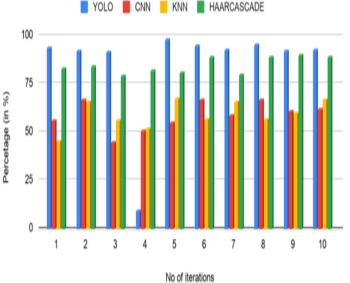
\includegraphics[width=\linewidth]{images/yolo_comp/yolo_acc_perf.png}
        \caption{Genauigkeitsperformance verschiedener Objektdetektoren in verschiedenen Iterationen \cite{Pavani2022}}
        \label{Scr:comp_object_detectorAcc}
    \end{subfigure}
    \hfill
    \begin{subfigure}[b]{0.45\textwidth}
        \centering
        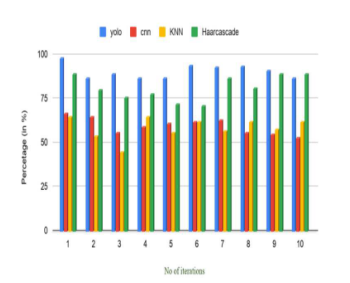
\includegraphics[width=\linewidth]{images/yolo_comp/yolo_prec_perf.png}
        \caption{Präzisionsperformance verschiedener Objektdetektoren in verschiedenen Iterationen  \cite{Pavani2022}}
        \label{Scr:comp_object_detectorPrec}
    \end{subfigure} 
    \caption[Vergleich von verschiedenen Objektdetektionsalgorithmen (YOLO, CNN, KNN, Haarcascade)]{Vergleich von verschiedenen Objektdetektionsalgorithmen (YOLO, CNN, KNN, Haarcascade); die Werte von YOLO sind relativ konstant über alle 10 Iterationen \cite{Pavani2022}}
    \label{Scr:comp_object_detector}
\end{figure}
  
    \begin{figure}[h]
		\centering
		\includegraphics*[scale = 0.4, keepaspectratio]{images/YOLO/YOLO_loss_function_detail_expl.png}
		\caption[Detaillierte Erklärung der YOLO Loss Funktion]{Detaillierte Erklärung der YOLO Loss Funktion\citep{Terven2023}}
		\label{YOLO_loss_function_detail}
 	\end{figure}


     \begin{figure}
        \begin{multline}
            \lambda_{coord} \sum_{i=0}^{s^2} \sum_{j=0}^{B} \mathbb{1}_{i j}^{obj}\left[(x_i-\hat{x}_i)^2 + (y_i - \hat{y}_i)^2\right]\\
            + \lambda_{coord} \sum_{i=0}^{s^2} \sum_{j=0}^{B} \mathbb{1}_{i j}^{obj}\left[\left(\sqrt{w_i} - \sqrt{\hat{w_i}}\right)^2 + \left(\sqrt{h_i}-\sqrt{\hat{h_i}}\right)^2\right]\\
            + \sum_{i=0}^{s^2} \sum_{j=0}^{B} \mathbb{1}_{i j}^{obj}\left(C_i - \hat{C_i}\right)^2\\
            + \lambda_{coord} \sum_{i=0}^{s^2} \sum_{j=0}^{B} \mathbb{1}_{i j}^{obj}\left(C_i - \hat{C_i}\right)^2\\
            + \sum_{i=0}^{s^2} \mathbb{1}_{i j}^{obj} \sum_{c \in classes } \left(p_i(c)-\hat{p_i}(c)\right)^2
        \end{multline} 
        \caption{Mehrteilige Verlustfunktion, die von YOLO während des Trainings optimiert wird \citep{Redmon2016}}
        \label{YOLO_Loss_function}
    \end{figure}

    
	
	

    \begin{figure}[h]
		\centering
		\includegraphics*[scale = 0.15, keepaspectratio]{images/YOLO/YOLO_timeline_vers.png}
		\caption[Übersicht über verschiedene YOLO Versionen im Zeitverlauf]{Übersicht über verschiedene YOLO-Versionen im Zeitverlauf \citep{Terven2023}}
		\label{YOLO_timeline_vers}
		\end{figure}

    \begin{figure}[h]
        \centering
        \includegraphics*[scale = 0.35, keepaspectratio]{images/YOLO/YOLOv8_Arch.png}
        \caption[Die Architektur von YOLOv8]{Die Architektur von YOLOv8 \citep{Terven2023}}
        \label{YOLOv8_Arch}
    \end{figure}
    \clearpage
    \subsection{Formverarbeitung}
    \begin{figure}[ht]
        \centering
        \includegraphics*[scale = 0.65, keepaspectratio, trim=2 2 2 2 ]{images/DCE/schem_maps_paper_DCE.png}
        \caption[Anwendungsbeispiele für die \glqq Discrete Curve Evolution\grqq{}]{Anwendungsbeispiele für die \glqq Discrete Curve Evolution\grqq{}  \citep{Barkowsky2000}.}
        \label{Bsp_DCE_Bark_Paper}
    \end{figure}


    \begin{figure}[ht]
		\centering
		\begin{subfigure}[b]{0.30\textwidth}
			\frame{
\includegraphics[width=\textwidth]{images/DCE/kleines Beispiel erweitert/testpng0.png}}
            \caption{Polygon ohne Vereinfachung}
		\end{subfigure} 
		\begin{subfigure}[b]{0.30\textwidth}
            \frame{
			
\includegraphics[width=\textwidth]{images/DCE/kleines Beispiel erweitert/testpng419.png}}
            \caption{Polygon (80 Punkte) }
		\end{subfigure}
        \begin{subfigure}[b]{0.30\textwidth}
			\frame{
\includegraphics[width=\textwidth]{images/DCE/kleines Beispiel erweitert/testpng429.png}}
            \caption{Polygon (70 Punkte)}
		\end{subfigure}
        \begin{subfigure}[b]{0.30\textwidth}
			\frame{
\includegraphics[width=\textwidth]{images/DCE/kleines Beispiel erweitert/testpng439.png}}
            \caption{Polygon (60 Punkte)}
		\end{subfigure}
        \begin{subfigure}[b]{0.30\textwidth}
			\frame{
\includegraphics[width=\textwidth]{images/DCE/kleines Beispiel erweitert/testpng449.png}}
            \caption{Polygon (50 Punkte)}
		\end{subfigure}
        \begin{subfigure}[b]{0.30\textwidth}
			\frame{
\includegraphics[width=\textwidth]{images/DCE/kleines Beispiel erweitert/testpng459.png}}
            \caption{Polygon (40 Punkte)}
		\end{subfigure}
        \begin{subfigure}[b]{0.30\textwidth}
			\frame{
\includegraphics[width=\textwidth]{images/DCE/kleines Beispiel erweitert/testpng469.png}}
            \caption{Polygon (30 Punkte)}
		\end{subfigure}
        \begin{subfigure}[b]{0.30\textwidth}
			\frame{
\includegraphics[width=\textwidth]{images/DCE/kleines Beispiel erweitert/testpng479.png}}
            \caption{Polygon (20 Punkte)}
		\end{subfigure}
        \begin{subfigure}[b]{0.30\textwidth}
			\frame{
\includegraphics[width=\textwidth]{images/DCE/kleines Beispiel erweitert/testpng489.png}}
            \caption{Polygon (10 Punkte)}
		\end{subfigure}
		\caption[Anwendungsbeispiel für DCE aus eigenen Daten]{Anwendungsbeispiel für die DCE anhand eines Teilumrisses von Nordrhein Westfalen; (a) zeigt das Ursprungspolygon mit 499 Punkten; (b) bis (i) zeigen um je 10 Punkte reduzierte Polygone, von 80 Punkten bis 10 Punkten (Quelle: eigene Darstellung)}
		\label{Scr:DCE_test_run_nrw}
	\end{figure}





    \clearpage
\subsection{Evaluation}{

    \begin{figure}[ht]

        \begin{subfigure}[b]{0.65\textwidth}
            \centering
            \includegraphics[width=\linewidth]{images/comp_pictures_settings/Scr_RAW.png}
            \caption{Screenshot aus dem 10-sekündigem Testdatensatz bei Frame 01:00:08:12}
        \end{subfigure} \hfill
        \begin{subfigure}[b]{0.65\textwidth}
            \centering
            \includegraphics[width=\linewidth]{images/comp_pictures_settings/Scr2_BB.png}
            \caption{Screenshot aus dem 30-sekündigem Testdatensatz bei Frame 01:00:08:12}
        \end{subfigure}
        \centering
        \begin{subfigure}[b]{0.65\textwidth}
            \centering
            \includegraphics[width=\linewidth]{images/comp_pictures_settings/Scr2_FB.png}
            \caption{Screenshot aus dem analysierten 10-sekündigem Testdatensatz bei Frame 01:00:08:12}
        \end{subfigure}
        \caption[Screenshots aus dem 10- und 30-sekündigen Testdatensätzen]{Screenshots aus dem 10- und 30-sekündigen Testdatensätzen. (a) zeigt die Testdaten ohne Bearbeitung; (b) zeigt den gleichen Frame aus dem 30-sekündigen Testdatensatz, der mit YOLO analysiert und von der DCE vereinfacht wurde, es wurden jedoch nur die Boundingboxen der erkannten Objekte schwarz gerendert; (c) zeigt den gleichen Frame aus dem 10-sekündigen Testdatensatz, hier wurde das gesamte Frame außer der vereinfachten Umrisse der detektierten Objekte schwarz gerendert (Quelle: eigene Darstellung)}
        \label{Scr:Settings_Comp}
    \end{figure} 
\clearpage
\begin{table}[h]
    \centering
\caption[Vergleich der verschiedenen YOLO Modelle bei 1 Sekunde Video (30 Frames)]{Vergleich der verschiedenen YOLO Modelle bei 1 Sekunde Video (30 Frames) (Quelle: eigene Darstellung; \ref{cd:listing_A1s_EF_results.txt(Y8n)}; \ref{cd:listing_A1s_RV_results.txt(Y8n)}; \ref{cd:listing_A1s_EF_results.txt(Y8m)}; \ref{cd:listing_A1s_RV_results.txt(Y8m)}; \ref{cd:listing_A1s_EF_results.txt(Y8x)}; \ref{cd:listing_A1s_RV_results.txt(Y8x)})}
\label{tab:YOLO8_A1s}
\begin{tabular}{l|l|l|l|l|l|l}
    & \textbf{8n (EF)} & \textbf{8n (RV)} & \textbf{8m (EF)} & \textbf{8m (RV)} & \textbf{8x (EF)} & \textbf{8x (RV)} \\ \hline
\textit{\begin{tabular}[c]{@{}l@{}}Anzahl Punkte/Winkel\\ vor DCE\end{tabular}} & 5.353 & 5.303 & 5.863 & 5.885 & 5.306 & 5.325 \\ \hline
\textit{\begin{tabular}[c]{@{}l@{}}Anzahl Punkte/Winkel\\ nach DCE\end{tabular}} & 1.919 & 1.880 & 2.168 & 2.185 & 1.965 & 1.988 \\ \hline
\textit{\begin{tabular}[c]{@{}l@{}}Anzahl vergl. Winkel\\ bei SSM Berechnung\end{tabular}} & 19.100 & 17.811 & 10.251 & 10.130 & 11.803 & 11.858 \\ \hline
\textit{} &  &  &  &  &  &  \\ \hline
\textit{\begin{tabular}[c]{@{}l@{}}Gesamtwinkelsumme\\ (in Deg.)\end{tabular}} & 6.020,32 & 5.898,2 & 6.802,79 & 6.856,27 & 6.166,18 & 6.238,21 \\ \hline
\textit{erkannte Polygone} & 147 & 145 & 209 & 210 & 212 & 214 \\ \hline
\textit{verglichene Polygone} & 131 & 129 & 188 & 189 & 193 & 194 \\ \hline
\textit{Prozessierungszeit (in Sek.)} & 29,54 & 20,19 & 47,92 & 30.64 & 80,15 & 44,09
\end{tabular}
\end{table}


    \begin{table}[ht]
        \centering
		\caption[Vergleich der SSMs bei verschiedenen YOLO Modellen bei 1 Sekunde Video (30 Frames)]{Vergleich der SSMs bei verschiedenen YOLO Modellen bei 1 Sekunde Video (30 Frames) (Quelle: eigene Darstellung; \ref{cd:listing_A1s_EF_results.txt(Y8n)}; \ref{cd:listing_A1s_RV_results.txt(Y8n)}; \ref{cd:listing_A1s_EF_results.txt(Y8m)}; \ref{cd:listing_A1s_RV_results.txt(Y8m)}; \ref{cd:listing_A1s_EF_results.txt(Y8x)}; \ref{cd:listing_A1s_RV_results.txt(Y8x)})}
		\label{tab:YOLO8_A1s_SSM}
		\begin{tabular}{l|l|l|l|l|l|l}
		 & \textbf{8n (EF)} & \textbf{8n (RV)} & \textbf{8m (EF)} & \textbf{8m (RV)} & \textbf{8x (EF)} & \textbf{8x (RV)} \\ \hline
		\textit{Absolute SSM Auto} & 2,0174 & 2,0174 & 2,2393 & 2,3659 & 3,8058 & 4,1018 \\ \hline
		\textit{SSM pro Fr. und Kl. Auto} & 0,0672 & 0,0672 & 0,0746 & 0,0789 & 0,1269 & 0,1637 \\ \hline
		\textit{SSM pro detektiertes Auto} & 0,0672 & 0,0721 & 0,0622 & 0,0676 & 0,0634 & 0,0672 \\ \hline
		\textit{\begin{tabular}[c]{@{}l@{}}absolute Anz. detektierter\\ Autos (in Klam. pro Fr.)\end{tabular}} & \begin{tabular}[c]{@{}l@{}}30\\ (1,00)\end{tabular} & \begin{tabular}[c]{@{}l@{}}28\\ (0,93)\end{tabular} & \begin{tabular}[c]{@{}l@{}}36\\ (1,2)\end{tabular} & \begin{tabular}[c]{@{}l@{}}35\\ (1,17)\end{tabular} & \begin{tabular}[c]{@{}l@{}}60\\ (2,00)\end{tabular} & \begin{tabular}[c]{@{}l@{}}61\\ (2,23)\end{tabular} \\ \hline
		 &  &  &  &  &  &  \\ \hline
		\textit{Absolute SSM LKW} & 4,4640 & 4,6617 & 13,3996 & 14,2144 & 11,5296 & 11,8367 \\ \hline
		\textit{SSM pro Fr. und Kl. LKW} & 0,1488 & 0,1554 & 0,4467 & 0,4738 & 0,3843 & 0,3946 \\ \hline
		\textit{SSM pro detektierter LKW} & 0,2349 & 0,2454 & 0,2197 & 0,2330 & 0,1696 & 0,1767 \\ \hline
		\textit{\begin{tabular}[c]{@{}l@{}}absolute Anz. detektierter\\ LKW (in Klam. pro Fr.)\end{tabular}} & \begin{tabular}[c]{@{}l@{}}19\\ (0,63)\end{tabular} & \begin{tabular}[c]{@{}l@{}}19\\ (0,63)\end{tabular} & \begin{tabular}[c]{@{}l@{}}61\\ (2,03)\end{tabular} & \begin{tabular}[c]{@{}l@{}}61\\ (2,03)\end{tabular} & \begin{tabular}[c]{@{}l@{}}68\\ (2,27)\end{tabular} & \begin{tabular}[c]{@{}l@{}}67\\ (2,23)\end{tabular} \\ \hline
		 &  &  &  &  &  &  \\ \hline
		\textit{Absolute SSM Zug} & 11,8231 & 11,8231 &  &  &  &  \\ \hline
		\textit{SSM pro Fr. und Kl. Zug} & 0,3941 & 0,3941 &  &  &  &  \\ \hline
		\textit{SSM pro detektierten Zug} & 0,3111 & 0,3378 &  &  &  &  \\ \hline
		\textit{\begin{tabular}[c]{@{}l@{}}absolute Anz. detektierter\\ Züge (in Klam. pro Fr.)\end{tabular}} & \begin{tabular}[c]{@{}l@{}}38\\ (1,27)\end{tabular} & \begin{tabular}[c]{@{}l@{}}35\\ (1,17)\end{tabular} &  &  &  &  \\ \hline
		 &  &  &  &  &  &  \\ \hline
		\textit{Absolute SSM Bus} &  &  & 1,8576 & 1,8576 &  &  \\ \hline
		\textit{SSM pro Fr. und Kl. Bus} &  &  & 0,0619 & 0,0619 &  &  \\ \hline
		\textit{SSM pro detektiertem Bus} &  &  & 0,4644 & 0,4644 &  &  \\ \hline
		\textit{\begin{tabular}[c]{@{}l@{}}absolute Anz. detektierter\\ Busse (in Klam. pro Fr.)\end{tabular}} &  &  & \begin{tabular}[c]{@{}l@{}}4\\ (0,13)\end{tabular} & \begin{tabular}[c]{@{}l@{}}4\\ (0,13)\end{tabular} &  & 
		\end{tabular}
		\end{table}
        \clearpage

        \subsubsection{Geringe und hohe DCE Substitionslimits}
            \begin{table}[ht]
                \centering
                \caption[Vergleich der Basisdaten bei 1 Sekunde Video (30 Frames) und verschiedenen DCE Substitutionslimits]{Vergleich der Basisdaten bei 1 Sekunde Video (30 Frames) und verschiedenen DCE Substitutionslimits (Quelle: eigene Darstellung; \ref{cd:listing_A1s_RV_minor_results.txt(Y8x)}, \ref{cd:listing_A1s_RV_more_results.txt(Y8x)})}
                \label{tab:YOLO8_minor_more_DCE_A1s}
                \begin{tabular}{l|l|l|l}
                    & \textbf{\begin{tabular}[c]{@{}l@{}}geringe DCE\\ Punktgrenzen\end{tabular}} & \textbf{Referenz} & \textbf{\begin{tabular}[c]{@{}l@{}}hohe DCE\\ Punktgrenzen\end{tabular}} \\ \hline
                   \textit{\begin{tabular}[c]{@{}l@{}}Anzahl Punkte/Winkel \\ vor DCE\end{tabular}} & 5.325 & 5.325 & 5.325 \\ \hline
                   \textit{\begin{tabular}[c]{@{}l@{}}Anzahl Punkte/Winkel\\ nach DCE\end{tabular}} & 1.174 & 1.988 & 4.026 \\ \hline
                   \textit{\begin{tabular}[c]{@{}l@{}}Anzahl vergl. Winkel\\ bei SSM Berechnung\end{tabular}} & 3.987 & 11.858 & 74.312 \\ \hline
                   \textit{} &  &  &  \\ \hline
                   \textit{Gesamtwinkelsumme} & 3.688,93 & 6.238,21 & 12.630,05 \\ \hline
                   \textit{erkannte Polygone} & 214 & 214 & 214 \\ \hline
                   \textit{verglichene Polygone} & 194 & 194 & 194 \\ \hline
                   \textit{Prozessierungszeit (in Sek.)} & 45,24 & 44,09 & 43,45
                   \end{tabular}
                \end{table}
    
                \begin{table}[ht]
                    \caption[Vergleich der SSMs bei verschiedenen DCE Substitionslimits bei einem 1-sekündigem Video (30 Frames) ]{Vergleich der SSMs bei verschiedenen DCE Substitionslimits bei einem 1-sekündigem Video (30 Frames) (Quelle: eigene Darstellung; \ref{cd:listing_A1s_RV_minor_results.txt(Y8x)}, \ref{cd:listing_A1s_RV_more_results.txt(Y8x)})}
                    \label{tab:Minor_More_DCE_SSMs_A1s}
                    \centering
                    \begin{tabular}{l|l|l|l}
                        & \textbf{\begin{tabular}[c]{@{}l@{}}geringe DCE\\ Punktgrenzen\end{tabular}} & \textbf{Referenz} & \textbf{\begin{tabular}[c]{@{}l@{}}hohe DCE\\ Punktgrenzen\end{tabular}} \\ \hline
                       \textit{Absolute SSM Auto} & 3,0831 & 4,1018 & 7,7453 \\ \hline
                       \textit{SSM pro Fr. und Kl. Auto} & 0,1028 & 0,1367 & 0,2582 \\ \hline
                       \textit{SSM pro detektiertes Auto} & 0,0505 & 0,0672 & 0,1270 \\ \hline
                       \textit{\begin{tabular}[c]{@{}l@{}}absolute Anz. detektierter\\ Autos (in Kl. pr. Fr.)\end{tabular}} & \begin{tabular}[c]{@{}l@{}}61\\ (2,03)\end{tabular} & \begin{tabular}[c]{@{}l@{}}61\\ (2,03)\end{tabular} & \begin{tabular}[c]{@{}l@{}}61\\ (2,03)\end{tabular} \\ \hline
                       \textit{} &  &  &  \\ \hline
                       \textit{Absolute SSM LKW} & 9,4661 & 11,8367 & 22,6788 \\ \hline
                       \textit{SSM pro Fr. und Kl. LKW} & 0,3155 & 0,3946 & 0,7560 \\ \hline
                       \textit{SSM pro detektierten LKW} & 0,1413 & 0,1767 & 0,3385 \\ \hline
                       \textit{\begin{tabular}[c]{@{}l@{}}Absolute Anz. detektierter\\ LKW (in Kl. pro Fr.)\end{tabular}} & \begin{tabular}[c]{@{}l@{}}67\\ (2,23)\end{tabular} & \begin{tabular}[c]{@{}l@{}}67\\ (2,23)\end{tabular} & \begin{tabular}[c]{@{}l@{}}67\\ (2,23)\end{tabular}
                       \end{tabular}
                    \end{table}	
                    
                
            
}
}
\clearpage
\lstset{commentstyle=\color{black}, stepnumber=2, basicstyle=\ttfamily\scriptsize} 
\section{Listing der Evaluationsergebnisse}
\subsection{Listing der Result Textdaten für YOLO8n Testdurchläufe}{ \label{ls:result_txts}
    \lstinputlisting[caption={Statistikdatei zu A1s\_EF\_results.txt (YoloV8n)}, label = {cd:listing_A1s_EF_results.txt(Y8n)}, language={}]{../Code/vid_examples/evaluation/01Yolo8n/A1s_EF_results.txt}
    \lstinputlisting[caption={Statistikdatei zu A1s\_RV\_results.txt (YoloV8n)}, label = {cd:listing_A1s_RV_results.txt(Y8n)}, language={}]{../Code/vid_examples/evaluation/01Yolo8n/A1s_RV_results.txt}
    \lstinputlisting[caption={Statistikdatei zu A10s\_EF\_results.txt (YoloV8n)}, label = {cd:listing_A10s_EF_results.txt(Y8n)}, language={}]{../Code/vid_examples/evaluation/01Yolo8n/A10s_EF_results.txt}
    \lstinputlisting[caption={Statistikdatei zu A10s\_RV\_results.txt (YoloV8n)}, label = {cd:listing_A10s_RV_results.txt(Y8n)}, language={}]{../Code/vid_examples/evaluation/01Yolo8n/A10s_RV_results.txt}
}
\subsection{Listing der Result Textdaten für YOLO8m Testdurchläufe}{
    \lstinputlisting[caption={Statistikdatei zu A1s\_EF\_results.txt (YoloV8m)}, label = {cd:listing_A1s_EF_results.txt(Y8m)}, language={}]{../Code/vid_examples/evaluation/02Yolo8m/A1s_EF_results.txt}
    \lstinputlisting[caption={Statistikdatei zu A1s\_RV\_results.txt (YoloV8m)}, label = {cd:listing_A1s_RV_results.txt(Y8m)}, language={}]{../Code/vid_examples/evaluation/02Yolo8m/A1s_RV_results.txt}
    \lstinputlisting[caption={Statistikdatei zu A10s\_EF\_results.txt (YoloV8m)}, label = {cd:listing_A10s_EF_results.txt(Y8m)}, language={}]{../Code/vid_examples/evaluation/02Yolo8m/A10s_EF_results.txt}
    \lstinputlisting[caption={Statistikdatei zu A10s\_RV\_results.txt (YoloV8m)}, label = {cd:listing_A10s_RV_results.txt(Y8m)}, language={}]{../Code/vid_examples/evaluation/02Yolo8m/A10s_RV_results.txt}
}
\subsection{Listing der Result Textdaten für YOLO8x Testdurchläufe}{
    \lstinputlisting[caption={Statistikdatei zu A1s\_EF\_results.txt (YoloV8x)}, label = {cd:listing_A1s_EF_results.txt(Y8x)}, language={}]{../Code/vid_examples/evaluation/03Yolo8x/A1s_EF_results.txt}
    \lstinputlisting[caption={Statistikdatei zu A1s\_RV\_results.txt (YoloV8x)}, label = {cd:listing_A1s_RV_results.txt(Y8x)}, language={}]{../Code/vid_examples/evaluation/03Yolo8x/A1s_RV_results.txt}
    \lstinputlisting[caption={Statistikdatei zu A10s\_EF\_results.txt (YoloV8x)}, label = {cd:listing_A10s_EF_results.txt(Y8x)}, language={}]{../Code/vid_examples/evaluation/03Yolo8x/A10s_EF_results.txt}
    \lstinputlisting[caption={Statistikdatei zu A10s\_RV\_results.txt (YoloV8x)}, label = {cd:listing_A10s_RV_results.txt(Y8x)}, language={}]{../Code/vid_examples/evaluation/03Yolo8x/A10s_RV_results.txt}
}
\subsection{Listing der Result Textdaten der weiteren Testfälle}{
    \subsubsection{Schiffstracking}{
        \lstinputlisting[caption={Statistikdatei zu S1s\_RV\_10.txt (YoloV8x, Schiffstracking)}, label = {cd:listing_A1s_RV_shiptracking_results.txt(Y8x)}, language={}]{../Code/vid_examples/evaluation/weitere_testfaelle/shiptracking/A1s_RV_10.txt}
        \lstinputlisting[caption={Statistikdatei zu S21s\_RV\_10.txt (YoloV8x, Schiffstracking)}, label = {cd:listing_A21s_RV_shiptracking_results.txt(Y8x)}, language={}]{../Code/vid_examples/evaluation/weitere_testfaelle/shiptracking/A21s_RV_10.txt}
    }
    \subsubsection{Geringe und hohe DCE Substitionslimits}{
        \lstinputlisting[caption={Statistikdatei zu A1s\_RV\_minor.txt (YoloV8x, geringes DCE Substitionslimit)}, label = {cd:listing_A1s_RV_minor_results.txt(Y8x)}, language={}]{../Code/vid_examples/evaluation/weitere_testfaelle/minor_more_DCEPoints/A1s_RV_minor.txt}  
        \lstinputlisting[caption={Statistikdatei zu A1s\_RV\_more.txt (YoloV8x, hohes DCE Substitionslimit)}, label = {cd:listing_A1s_RV_more_results.txt(Y8x)}, language={}]{../Code/vid_examples/evaluation/weitere_testfaelle/minor_more_DCEPoints/A1s_RV_more.txt}     
        \lstinputlisting[caption={Statistikdatei zu A10s\_RV\_minor.txt (YoloV8x, geringes DCE Substitionslimit)}, label = {cd:listing_A10s_RV_minor_results.txt(Y8x)}, language={}]{../Code/vid_examples/evaluation/weitere_testfaelle/minor_more_DCEPoints/A10s_RV_minor.txt}  
        \lstinputlisting[caption={Statistikdatei zu A10s\_RV\_more.txt (YoloV8x, hohes DCE Substitionslimit)}, label = {cd:listing_A10s_RV_more_results.txt(Y8x)}, language={}]{../Code/vid_examples/evaluation/weitere_testfaelle/minor_more_DCEPoints/A10s_RV_more.txt} 

    }
   
    \subsubsection{Gleiche DCE Substitionslimits}{
        \lstinputlisting[caption={Statistikdatei zu A10s\_RV\_minorSame\_results.txt (YoloV8x, gleich wenige DCE Substitionslimits)}, label = {cd:listing_A10s_RV_minorSame_results.txt(Y8x)}, language={}]{../Code/vid_examples/evaluation/weitere_testfaelle/sameDCESubst/A10s_RV_minorSame_results.txt} 
        \lstinputlisting[caption={Statistikdatei zu A10s\_RV\_moreSame\_results.txt (YoloV8x, gleich hohe DCE Substitionslimits)}, label = {cd:listing_A10s_RV_moreSame_results.txt(Y8x)}, language={}]{../Code/vid_examples/evaluation/weitere_testfaelle/sameDCESubst/A10s_RV_moreSame_results.txt} 


    }
    \subsubsection{Langer Testdatensatz}{
        \lstinputlisting[caption={Statistikdatei zu A30s\_RV\_results.txt (YoloV8x, 30-sekündiger Testdatensatz)}, label = {cd:listing_A30s_RV_results.txt(Y8x)}, language={}]{../Code/vid_examples/evaluation/weitere_testfaelle/longshots/A30s_RV_results.txt}  

    }

}
\section{Listing mit Dokumentation und Kommentaren}{\label{cd:gesamt_listing}}





\subsection{Vollständiges Listing von main.py}{
    \lstinputlisting[caption={Gesamtlisting main.py}, label = {cd:listing_main.py}]{../Code/main.py}}

\subsection{Vollständiges Listing von yolo\_every\_frame.py}{
    \lstinputlisting[caption={Gesamtlisting Yolo\_every\_frame.py}, label = {cd:listing_yolo_every_frame_py}]{../Code/YOLO/yolo_every_frame.py}}

\subsection{Vollständiges Listing von yolo\_result\_version.py}{
    \lstinputlisting[caption={Gesamtlisting Yolo\_result\_version.py}, label = {cd:listing_yolo_result_version}]{../Code/YOLO/yolo_result_version.py}}

\subsection{Vollständiges Listing von yolo\_segmentation.py}{
    \lstinputlisting[caption={Gesamtlisting Yolo\_segementation.py}, label = {cd:listing_yolo_segmentation.py}]{../Code/YOLO/yolo_segmentation.py}}

\subsection{Vollständiges Listing von DCE.py}{
    \lstinputlisting[caption={Gesamtlisting DCE.py}, label = {cd:listing_DCE.py}]{../Code/DCE/DCE.py}}

\subsection{ Vollständiges Listing von shape\_similarity\_meas.py}{
    \lstinputlisting[caption={Gesamtlisting shape\_sim\_meas.py}, label = {cd:listing_shape_sim_meas.py}]{../Code/Shape_Similiarity/shape_sim_meas.py}
}


\cleardoubleoddemptypage

\listoffigures
\cleardoubleoddemptypage

\listoftables
\cleardoubleoddemptypage

\lstlistoflistings
\cleardoubleoddemptypage


\printbibliography
\cleardoubleoddemptypage
%!TEX root = ../thesis.tex
\chapter*{Plagiatserklärung des Studierenden}
Hiermit versichere ich, dass die vorliegende Arbeit über 
\begin{center}
\textit{\printtitle}
\end{center}
selbstständig von mir und ohne fremde Hilfe verfasst worden ist, dass keine anderen Quellen und Hilfsmittel als die angegebenen benutzt worden sind und dass die Stellen der Arbeit, die anderen Werken – auch elektronischen Medien – dem Wortlaut oder Sinn nach entnommen wurden, auf jeden Fall unter Angabe der Quelle als Entlehnung kenntlich gemacht worden sind. Mir ist bekannt, dass es sich bei einem Plagiat um eine Täuschung handelt, die gemäß der Prüfungsordnung sanktioniert werden kann.

\vspace{0.75cm}
\parbox{17em}{\hrulefill} \\
\printname, \printcity, 29.09.2023 \\
\vspace{0.5cm}



Ich erkläre mich mit einem Abgleich der Arbeit mit anderen Texten zwecks Auffindung von Übereinstimmungen sowie mit einer zu diesem Zweck vorzunehmenden Speicherung der Arbeit in einer Datenbank einverstanden. 

Ich versichere, dass ich die vorliegende Arbeit oder Teile daraus nicht anderweitig als Prüfungsarbeit eingereicht habe.



\vspace{0.75cm}
\parbox{17em}{\hrulefill} \\
\printname, \printcity, 29.09.2023




\end{document}
